% % %
% Recommended compilation method:
%  $ latexmk -pdf m5231142.tex 
%
% If you use 
%  $ latexmk -pdfdvi m5231142.tex
% then you must write `dvipdfmx' in option of \documentclass, i.e.,
%  \documentclass[12pt, a4paper, openany, dvipdfmx]{book}
%
% % %

% % % Document Type
% % % Ref.: http://www.biwako.shiga-u.ac.jp/sensei/kumazawa/tex/book.html
\documentclass[11pt, a4paper, openany]{book}

% % % Necessary
\usepackage{amssymb, amsmath, latexsym}  % For mathematics [Before hyperref]
\usepackage[setpagesize=false]{hyperref} % For inserting hyperlink [Before graphicx]
\usepackage{graphicx}                    % For inserting figure
\usepackage{subcaption}                  % For caption of figures and tables
\usepackage[usenames]{color}             % For coloring
\usepackage[shortlabels]{enumitem}       % For useful enumerate and itemize environment
\usepackage{comment}                     % For commenting multiline
\usepackage{cite}                        % For citing references [After hyperref]
\usepackage{url}                         % For inserting URL
\usepackage{acro}                        % For listing abbreviations and symbols
\usepackage{master}                      % For master thesis [After graphicx and color]

% % % Convenient for tables and emphasis
\usepackage{tabularx}       % For flexible table
\usepackage{multirow}       % For combining multi rows for table
\usepackage{colortbl}       % For coloring table
\usepackage{longtable}      % For long table across multiple pages
\usepackage[normalem]{ulem} % For flexible underline etc.
\usepackage{bxascmac}       % For framing multiline

% % % Option
\usepackage{siunitx}   % For using SI units
\usepackage{afterpage} % For inserting newpage
\usepackage{listings}  % For inserting programming code
\usepackage{docmute}   % For compilation of divided files
\usepackage{CJKutf8}   % Japanese

% % % Floating figure and table
\makeatletter
\newcommand{\figcaption}[1]{\def\@captype{figure}\caption{#1}}
\newcommand{\tblcaption}[1]{\def\@captype{table}\caption{#1}}
\makeatother

% % % Inserting Japanese sentence
\newcommand*{\Ja}[1]{%
  \begin{CJK}{UTF8}{ipxm}#1\end{CJK}}

% % % Configuration for hyperlink
\hypersetup{ %
	breaklinks=true, %
	colorlinks=false, %
	urlcolor=blue, %
	urlbordercolor={0 1 1}}

% % % Define Command
\newcommand{\bm}[1]{\mbox{\boldmath $#1$}}

% % % Re-define names

% % 論文題目     / Title
\title{Deep Reinforcement Learning in Forex Trading Using Metrics}
% % 著者名       / Author name
\author{HARUGUHCI Takuma}
% % 修了時期     / Year and month when you complete master course
\datestamp{March 2021} 
% % 主査名と職階 / Name and position of chief examiner
\mainreferee{LI Xiang}    
\mainrefereeposition{Associate Professor}
% % 副査名と職階 / Name and position of deputy examiner
\secondreferee{MORI Kazuyoshi}
\secondrefereeposition{Professor}
\thirdreferee{JING Lei}
\thirdrefereeposition{Senior Associate Professor}

% % You can define abbreviations and symbols, if any.
% % If you show lists of either abbreviations, symbols or both, 
% % you should define them in ./Chapter/Acronym.tex
% % However, if you do not need the lists, you should comment out the following line
% % and replace \showlist command to \showlists{y}{y}{n}{n}
% % % Reference: 
% http://tex.stackexchange.com/questions/86666/how-to-create-both-list-of-abbreviations-and-list-of-nomenclature-using-nomencl
% ftp://ftp.kddilabs.jp/CTAN/macros/latex/contrib/acro/acro_en.pdf
% % %

% Configuration for hyperlink and list of acronyms
\acsetup{hyperref=true, list-style=longtable, list-heading=chapter*}

% class `abbrev': abbreviations:
\DeclareAcronym{pc}{
  short = PC ,
  long  = Personal Computer ,
  class = abbrev
}
\DeclareAcronym{ws}{
  short = WS ,
  long  = Work Station ,
  class = abbrev
}
\DeclareAcronym{uoa}{
  short = UoA,
  long  = University of Aizu,
  class = abbrev
}

% class `nomencl': nomenclature (symbol)
\DeclareAcronym{A}{
  short = $\bm{A}$ ,
  long  = Matrix ,
  sort  = A ,
  class = nomencl
}
\DeclareAcronym{a}{
  short = $\bm{a}$ ,
  long  = Vector ,
  sort  = a ,
  class = nomencl
}
\DeclareAcronym{r}{
  short = $\mathbb{R}$ ,
  long  = Set of real numbers ,
  sort  = R ,
  class = nomencl
}



\begin{document}
% % タイトル、著作権、承認ページ、目次の作成 
% % Make pages for title, copyright, approval and table of contents
\makefrontmattar

% % 図、表、略語、記号一覧の表示
% % Show lists of figures, tables, abbreviations and symbols (Optional)
% % %
% % If you set 'n' to the fourth argument of \showlists{figures}{tables}{abbreviaions}{symbols}
% % (i.e. \showlists{y}{y}{y}{n}), list of symbols is not shown.
% % Similarly, you can decide if you show each list. 
% % %
\showlists{y}{y}{y}{y}
% \showlists{y}{y}{n}{n}

% % 謝辞を挿入 / Acknowledment (Optional)
\chapter*{Acknowledgment}
I express our sincere thanks to Prof. LI Xiang for helpful discussions and suggestions during COVID-19 pandemic. Also, Referees Prof. MORI Kazuyoshi and Prof. JING Lei gave me advice for my thesis. I also thank the lab members.
% % 要旨を挿入
\chapter*{Abstract}
% % There is no page number in abstract
\thispagestyle{empty}
In recent years, Deep Q-learning (DQL) becomes more and more important to any field. Deep Q-learning, which is also one of deep reinforcement learning (DRL), is Q-learning with Deep Q Network (DQN). Before employing reinforcement learning for finance in earnest, the papers that applied machine learning tended to focus on predicting the future. The weakness in the predictive approach is to ignore the option to wait. Therefore, this thesis studies DQN for the retail foreign exchange trading (Forex, A.K.A. FX). The DQN utilizes multiple moving averages (MA) of the exchange rate history like USD/JPY as state element. Based on the results, this thesis presented two conclusions. Firstly, unfortunately, the agent failed to learn to get profit in both training and testing because MA may be invalid metrics for Forex trading. Secondly, reinforcement learning itself was presumed to help to avoid losses. Accordingly, further investigation is needed to make this DQN method practical.



% % %
% Begin of Body
% % %
\configbody

% % When you request examiners to do peer review of your thesis, the paper should be double-spacing.
% % When you submit your thesis, the paper must be single-spacing.
\singlespacing
% \doublespacing

% % Chapterごとにファイルを分けて,それぞれをincludeする
% % You should make files of each chapter, and include them.
% % docmute package is convenient to edit and compile each file. If you are interested, please search the package.
\chapter{Introduction}
\section{Overview}
Foreign exchange is trading of currencies between two countries. For example, when a company in Japan imports some products from the U.S., it exchanges the yen into the U.S. dollar to pay.

In addition to importers and exporters, there are speculators in Forex markets. Individual traders of them often utilize the retail foreign exchange trading (Forex, A.K.A. FX). In Forex, expecting the exchange rate among currencies and taking the long or the short position, a trader tries to get the gain from the difference of the rate between present and future.

The long position is the buying position where he gets the profit if the rate rises (e.g., \$1=Y\llap{=}100 $\Longrightarrow$ \$1=Y\llap{=}120: Profit=Y\llap{=}20). In the opposite case, he suffers a loss. On the other hand, The short position is the selling position where he gets the profit if the rate decrease (e.g., \$1=Y\llap{=}100 $\Longrightarrow$ \$1=Y\llap{=}90 : Profit=Y\llap{=}10). In the opposite case, he suffers a loss. Taking no position is called the square, which means that you get no profit and suffer no loss.

Instead of prediction approach for the future rate, this paper focuses on the strategy to get the profit using Deep Q-learning. The contribution of the thesis is to confirm the performance of moving average as state in the learning because moving average is one of the most basic metrics in the Forex technical analysis.

This thesis has been organized as follows. The rest of this section describes Forex trading system, reinforcement learning, and research motivations. In Section \ref{sec:method_algo}, the algorithm and definitions about Deep Q-learning are detailed. In Section \ref{sec:experiment}, the way of the experiment, dataset, and the evaluation methods are detailed. Section \ref{sec:result} shows the results of the experiment and considers the meanings of them. In Section \ref{sec:conclusion}, conclusions are discussed.

\section{Forex Trading}
\subsection{Details of Forex System}
\label{sec:Forex}
\begin{figure}[htbp]
  \centering
  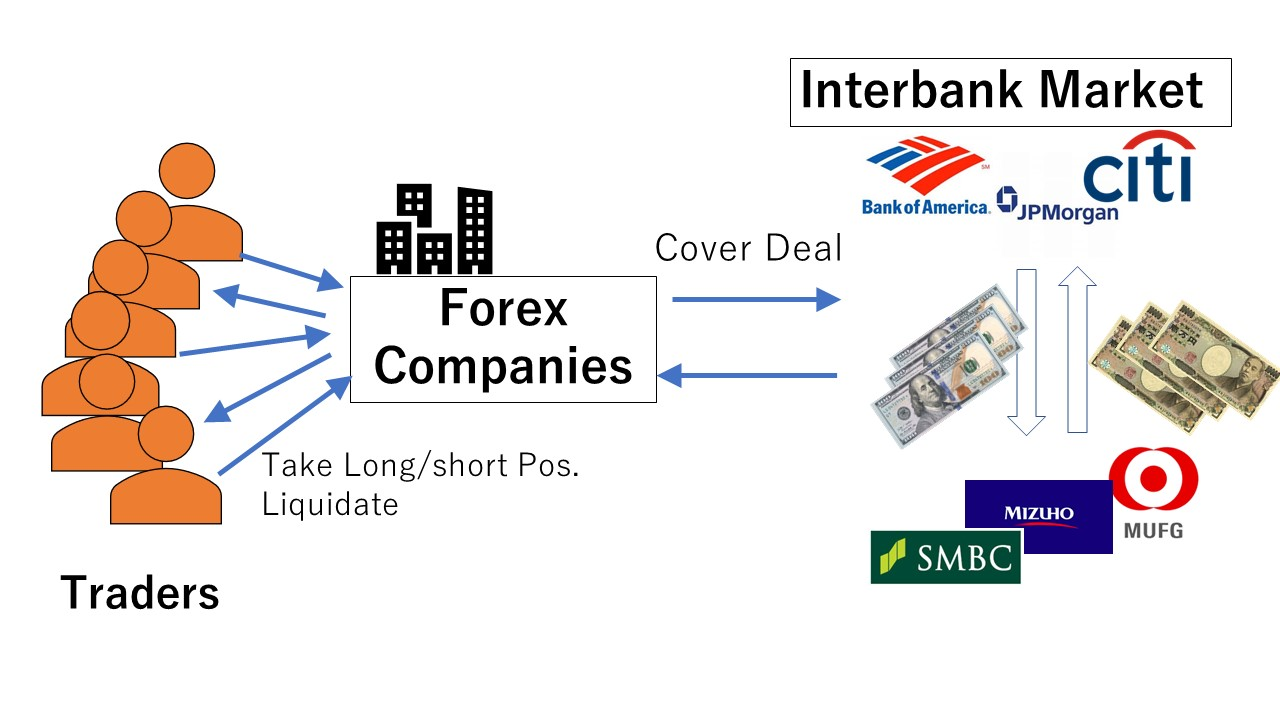
\includegraphics[scale=0.3]{./Figure/ForexEntity.jpg}
  \caption{The overview of Forex entities}
  \label{fig:entities}
\end{figure}
First, we look at the entities of Forex. In Figure \ref{fig:entities} that simplifies the actual situation \cite{bjr2016}, there are traders, Forex companies, and the interbank market. Traders order a Forex company to take a long/short position or to liquidate the position, and then the Forex company conducts the cover deal in the interbank market.

 Ignoring the revenue sources of the forex company such as transaction fee, let us consider the relationship among the long/short position, profit and loss (P/L), and the cover deal.

\begin{figure}
  \centering
  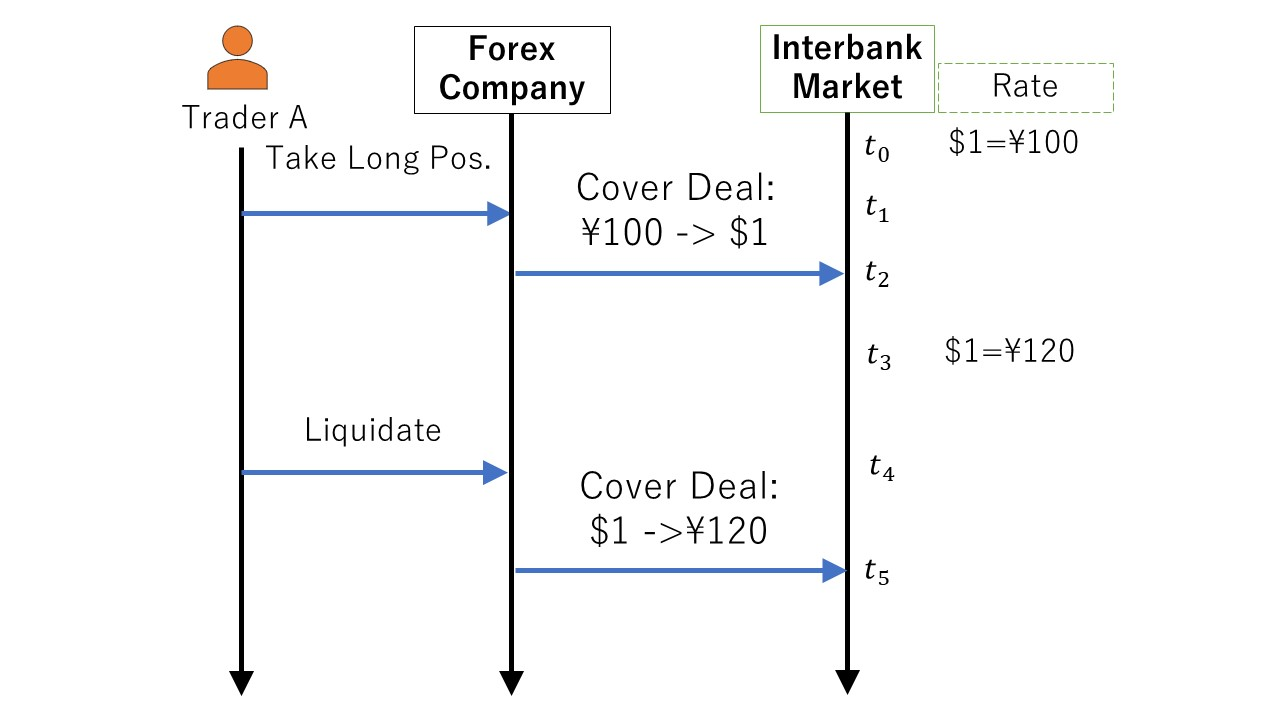
\includegraphics[scale=0.3]{./Figure/Long_CoverDeal1.jpg}
  \caption{Timeline for long position when getting profit}
  \label{fig:lcd1}
\end{figure}

\begin{table}
  \centering
  \caption{P/L and cover deal for long position when getting profit}
  \label{tb:lcd1}
  \begin{tabular}{|c|c|c|c|c|}
  \hline
  \multicolumn{1}{|c|}{} & \multicolumn{3}{c|}{Trader A} & \multicolumn{1}{c|}{} \\
  \cline{2-4}
  Time      & Position & Floating P/L & P/L        & Forex Capital \\
  \hline
  $ t_{0} $ & Square   & Y\llap{=}0   & Y\llap{=}0 & Y\llap{=}100 \\
  $ t_{1} $ & Long     & Y\llap{=}0   & Y\llap{=}0 & Y\llap{=}100 \\
  $ t_{2} $ & Long     & Y\llap{=}0   & Y\llap{=}0 & \$1          \\
  $ t_{3} $ & Long     &+Y\llap{=}20  & Y\llap{=}0 & \$1          \\
  $ t_{4} $ & Square   & Y\llap{=}0   &+Y\llap{=}20& \$1          \\
  $ t_{5} $ & Square   & Y\llap{=}0   &+Y\llap{=}20& Y\llap{=}120 - Y\llap{=}20 = Y\llap{=}100 \\
  \hline
  \end{tabular}
\end{table}

Figure \ref{fig:lcd1} shows that trader A makes a profit of Y\llap{=} 20 on taking the long position. When the trader takes the long position at time $ t_{1} $, the Forex company exchanges yens for dollars as cover deal at time $ t_{2} $. In general, the cover deal means the real trading in the interbank market corresponding to a trader’s position.

And then, suppose that the exchange rate \$1=Y\llap{=}100 changes to \$1=Y\llap{=}120 at time $ t_{3} $. The rate change brings the trader floating P/L. The floating P/L is unrealized profit or loss which floats (changes) in correspondence with the exchange rate and which position he has. For example, if the exchange rate \$1=Y\llap{=}120 at time $ t_{3} $ changes to \$1=Y\llap{=}110 at time $ t_{3.5} $ unlike Figure \ref{fig:lcd1}, his floating P/L as +Y\llap{=}20 also changes to +Y\llap{=}10.

At time $ t_{4} $, the trader liquidates his position to finally realize the profit as +Y\llap{=}20. Liquidating a position means changing the position into the square, finalizing his P/L. And then, the Forex company exchanges dollars for yen as cover deal at time $ t_{5} $ to pay the trader Y\llap{=}20.

There are four patterns for the taking positions and trader's P/L:
\begin{enumerate}
  \item Long position when getting profit $\Longrightarrow$ Figure \ref{fig:lcd1} and Table \ref{tb:lcd1}
  \item Long position when suffering loss $\Longrightarrow$ Figure \ref{fig:lcd2} and Table \ref{tb:lcd2}
  \item Short position when suffering loss $\Longrightarrow$ Figure \ref{fig:scd1} and Table \ref{tb:scd1}
  \item Short position when getting profit $\Longrightarrow$ Figure \ref{fig:scd2} and Table \ref{tb:scd2}
\end{enumerate}

Look at following figures and tables to understand all relationships among positions, P/L, and the cover deal.


\begin{figure}
  \centering
  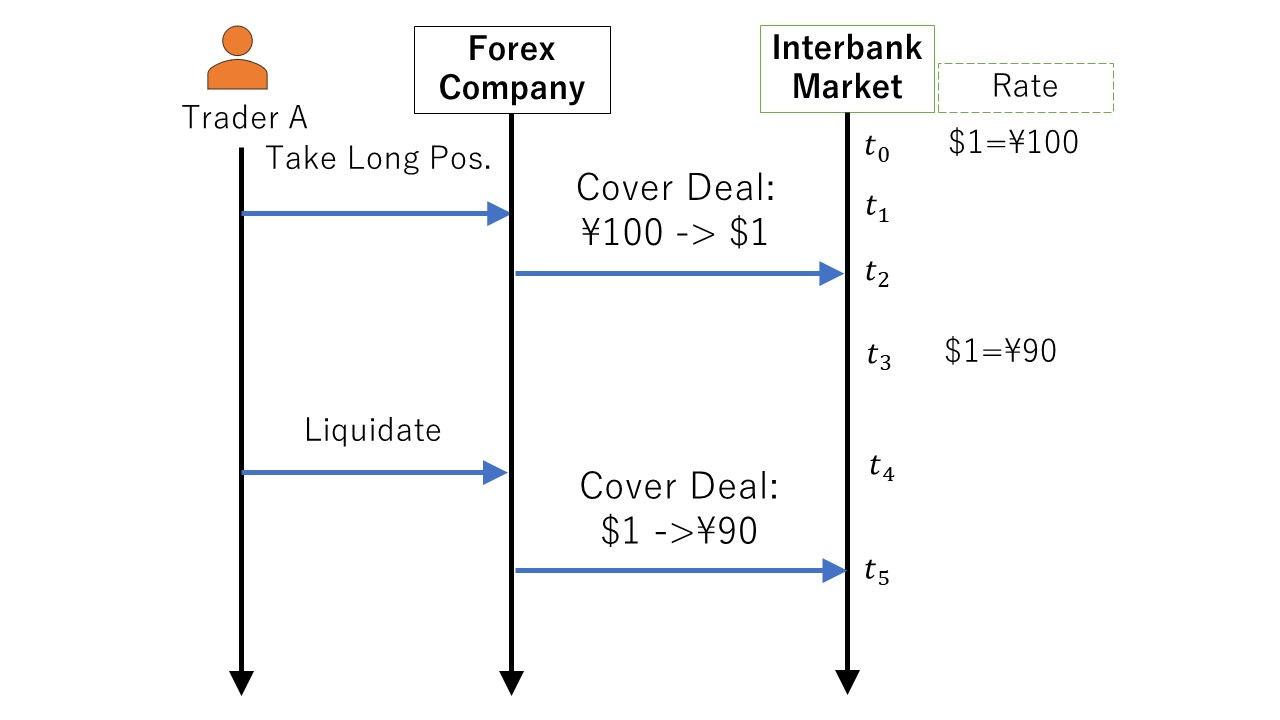
\includegraphics[scale=0.3]{./Figure/Long_CoverDeal2.jpg}
  \caption{Timeline for long position when suffering loss}
  \label{fig:lcd2}
\end{figure}

\begin{table}
  \centering
  \caption{P/L and cover deal for long position when suffering loss}
  \label{tb:lcd2}
  \begin{tabular}{|c|c|c|c|c|}
  \hline
  \multicolumn{1}{|c|}{} & \multicolumn{3}{c|}{Trader A} & \multicolumn{1}{c|}{} \\
  \cline{2-4}
  Time      & Position & Floating P/L & P/L        & Forex Capital   \\
  \hline
  $ t_{0} $ & Square   & Y\llap{=}0   & Y\llap{=}0 & Y\llap{=}100    \\
  $ t_{1} $ & Long     & Y\llap{=}0   & Y\llap{=}0 & Y\llap{=}100    \\
  $ t_{2} $ & Long     & Y\llap{=}0   & Y\llap{=}0 & \$1             \\
  $ t_{3} $ & Long     &-Y\llap{=}10  & Y\llap{=}0 & \$1             \\
  $ t_{4} $ & Square   & Y\llap{=}0   &-Y\llap{=}10& \$1             \\
  $ t_{5} $ & Square   & Y\llap{=}0   &-Y\llap{=}10& Y\llap{=}90 + Y\llap{=}10 = Y\llap{=}100 \\
  \hline
  \end{tabular}
\end{table}


\begin{figure}
  \centering
  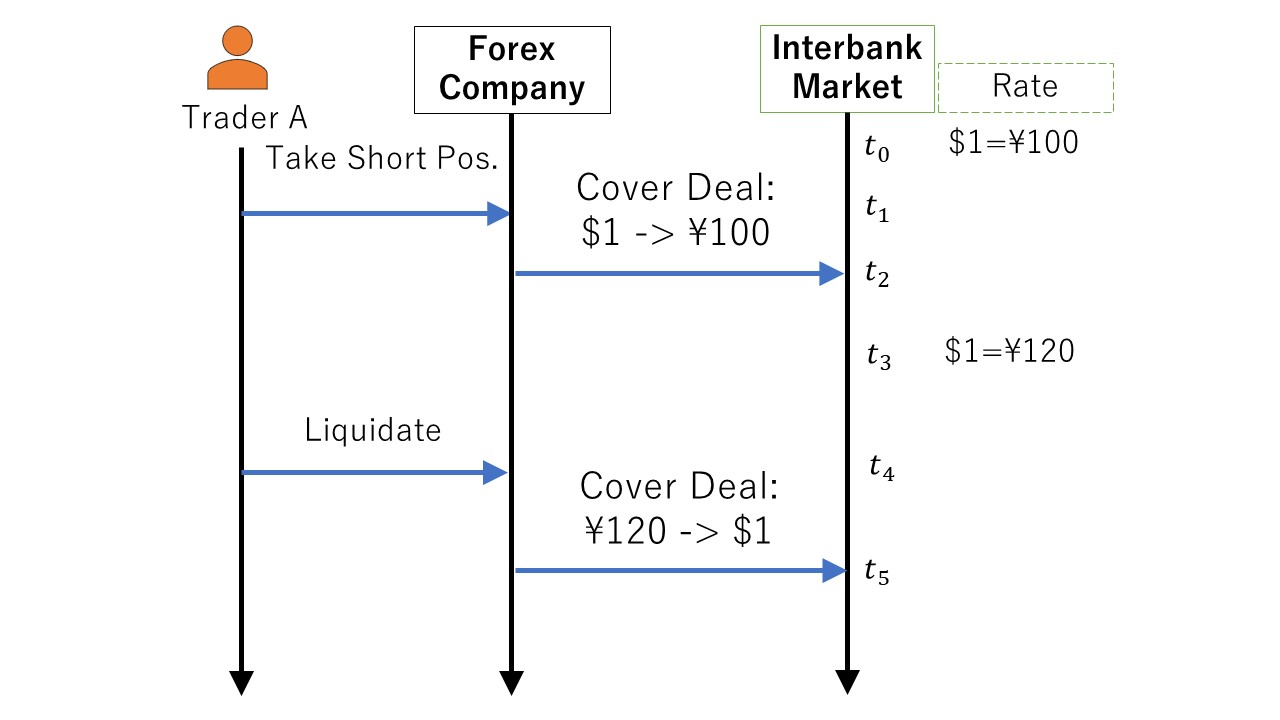
\includegraphics[scale=0.3]{./Figure/Short_CoverDeal1.jpg}
  \caption{Timeline for short position when suffering loss}
  \label{fig:scd1}
\end{figure}

\begin{table}
  \centering
  \caption{P/L and cover deal for short position when suffering loss}
  \label{tb:scd1}
  \begin{tabular}{|c|c|c|c|c|}
  \hline
  \multicolumn{1}{|c|}{} & \multicolumn{3}{c|}{Trader A} & \multicolumn{1}{c|}{} \\
  \cline{2-4}
  Time      & Position & Floating P/L & P/L        & Forex Capital \\
  \hline
  $ t_{0} $ & Square   & Y\llap{=}0   & Y\llap{=}0 & \$1           \\
  $ t_{1} $ & Short    & Y\llap{=}0   & Y\llap{=}0 & \$1           \\
  $ t_{2} $ & Short    & Y\llap{=}0   & Y\llap{=}0 & Y\llap{=}100  \\
  $ t_{3} $ & Short    &-Y\llap{=}20  & Y\llap{=}0 & Y\llap{=}100  \\
  $ t_{4} $ & Square   & Y\llap{=}0   &-Y\llap{=}20& Y\llap{=}100  \\
  $ t_{5} $ & Square   & Y\llap{=}0   &-Y\llap{=}20& Y\llap{=}100 + Y\llap{=}20 = \$1 \\
  \hline
  \end{tabular}
\end{table}


\begin{figure}
  \centering
  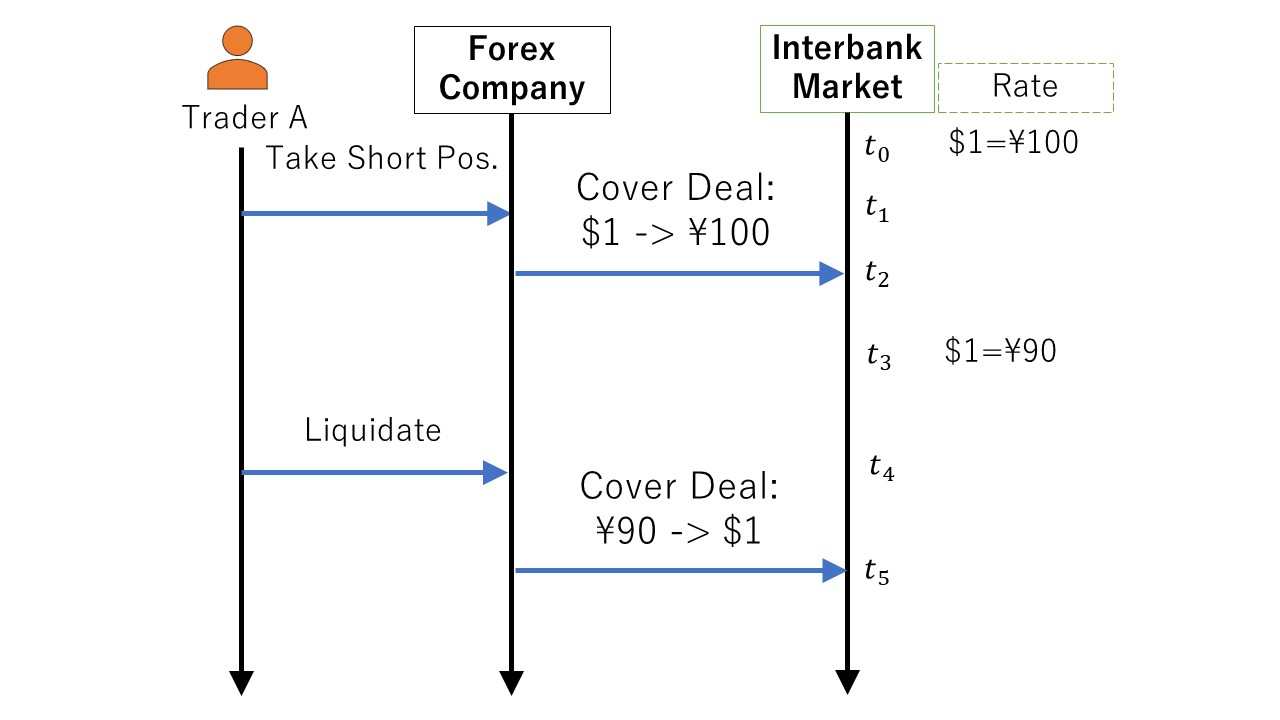
\includegraphics[scale=0.3]{./Figure/Short_CoverDeal2.jpg}
  \caption{Timeline for short position when getting profit}
  \label{fig:scd2}
\end{figure}

\begin{table}
  \centering
  \caption{P/L and cover deal for short position when getting profit}
  \label{tb:scd2}
  \begin{tabular}{|c|c|c|c|c|}
  \hline
  \multicolumn{1}{|c|}{} & \multicolumn{3}{c|}{Trader A} & \multicolumn{1}{c|}{} \\
  \cline{2-4}
  Time      & Position & Floating P/L & P/L        & Forex Capital   \\
  \hline
  $ t_{0} $ & Square   & Y\llap{=}0   & Y\llap{=}0 & \$1           \\
  $ t_{1} $ & Short    & Y\llap{=}0   & Y\llap{=}0 & \$1           \\
  $ t_{2} $ & Short    & Y\llap{=}0   & Y\llap{=}0 & Y\llap{=}100  \\
  $ t_{3} $ & Short    &+Y\llap{=}10  & Y\llap{=}0 & Y\llap{=}100  \\
  $ t_{4} $ & Square   & Y\llap{=}0   &+Y\llap{=}10& Y\llap{=}100  \\
  $ t_{5} $ & Square   & Y\llap{=}0   &+Y\llap{=}10& Y\llap{=}100 - Y\llap{=}10 = \$1 \\
  \hline
  \end{tabular}
\end{table}

The four patterns suggest two features. Firstly, the Forex company keeps the initial capital as Y\llap{=}100 or \$1 without any profit and any loss in any case. It shows that the cover deal literally covers the Forex company from the loss. 

Secondly, the position has the state transition as Figure \ref{fig:pos_trans}.

\begin{figure}[htbp]
  \centering
  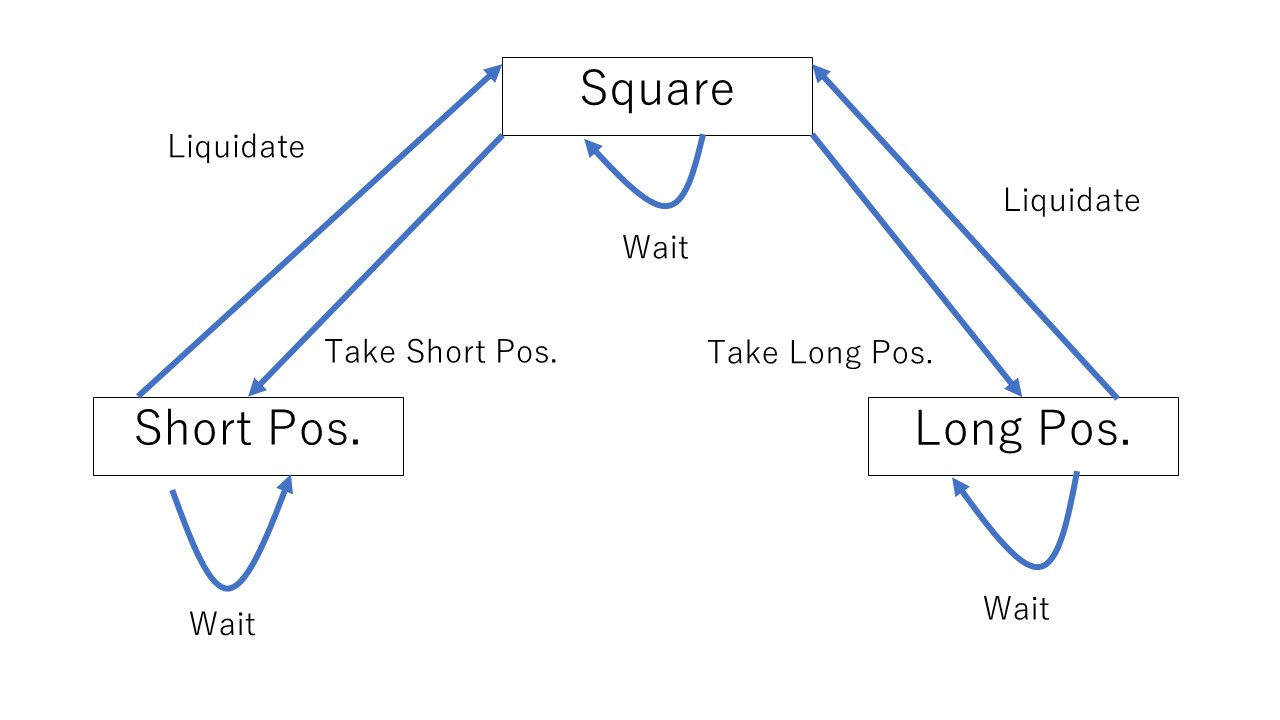
\includegraphics[scale=0.3]{./Figure/pos_transition.jpg}
  \caption{The diagram of the position state transition}
  \label{fig:pos_trans}
\end{figure}


\subsection{Simplification}
Within the scope of this research, all you have to do is to learn the below rules:
\begin{enumerate}
  \item Position State Transition as Figure \ref{fig:pos_trans}
  \item Position and floating P/L
  \begin{itemize}
    \item Long position: The dollar rate rises $\Longrightarrow$ Profit as floating P/L
    \item Long position: The dollar rate decreases $\Longrightarrow$ Loss as floating P/L
    \item Short position: The dollar rate rises $\Longrightarrow$ Loss as floating P/L
    \item Short position: The dollar rate decreases $\Longrightarrow$ Profit as floating P/L
  \end{itemize}
  \item The P/L is finally realized after liquidating the position. 
\end{enumerate}
You do not have to consider the Forex company because it does not affect the trader's P/L.

\section{Reinforcement Learning}
Reinforcement learning (RL) is one of machine learning which learns mapping the pairs of situations-to-actions so as to maximize a reward \cite{sutton2018rl}. In general, the reinforcement learning is modeled as Markov decision process (MDP) like Figure \ref{fig:rl}. At the very beginning, the agent receives the state $ S_{0} $ from the environment, and then the agent takes the action $ A_{0} $. The environment gives the agent the reward $ R_{1} $ and the state $ S_{1} $ in turn, and then the agent takes the action $ A_{1} $, and so on. The (\ref{eq:trajectory}) shows the trajectory: 

\begin{figure}[htbp]
  \centering
  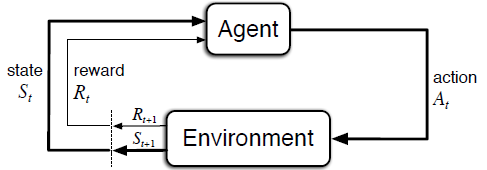
\includegraphics[scale=0.6]{./Figure/rl.png}
  \caption{The agent–environment interaction in a MDP \cite{sutton2018rl}}
  \label{fig:rl}
\end{figure}

\begin{equation}
  \label{eq:trajectory}
  S_{0}, A_{0}, R_{1}, S_{1}, A_{1}, R_{2}, S_{2}, A_{2}, ..., R_{T-1}, S_{T-1}, A_{T-1}, R_{T}, S_{T},
\end{equation}
where $T$ is a final time step \cite{sutton2018rl}. The range of time steps between $0$ and $T$ is called {\it episode} \cite{sutton2018rl}.


\section{Q-learning}
One of the methods in RL is Q-learning. Before explaining it, we introduce some related equations. First, let us define $q_{\pi}$ which is called {\it action-value function for policy} $\pi$ \cite{sutton2018rl} such as

\begin{equation}
  \label{eq:action-value_func}
  q_{\pi}(s,a) := \mathbb{E}[G_{t} | S_{t}=s, A_{t}=s].
\end{equation}

Equation (\ref{eq:action-value_func}) means that $q_{\pi}(s,a)$ outputs the expected return starting from state $s$ and taking the action $a$, after that following policy $\pi$. A policy $\pi$ is a rule where the agent determines the action, and the policy is calculated as conditional probability $\pi(a|s)$.

Second, we introduce {\it optimal action-value function} $q_{*}$, and define it as
\begin{equation}
  \label{eq:opt_av_func}
  q_{*}(s,a) := max \ q_{\pi}(s,a),
\end{equation}
for all $s \in \mathcal{S} $ and $a \in \mathcal{A}(s) $ where $\mathcal{S}$ is set of all nonterminal states and the $\mathcal{A}(s)$ is set of all actions available in state $s$ \cite{sutton2018rl}.

Third, based on Equation \ref{eq:opt_av_func}, it is known to be able to obtain the {\it Bellman optimality equation} for $q_{*}$ \cite{korekara} which is 
\begin{equation}
  \label{eq:Bellman_opt_eq}
  q_{*}(s,a) = \displaystyle \sum_{s'\in \mathcal{S}} p(s'|s,a)[r(s,a,s')+\gamma \ \underset{a' \in \mathcal{A}(s')}{max} \ q_{*}(s',a')].
\end{equation}
The $p(s'|s,a)$ is probability of transition to state $s'$, from state $s$ taking action $a$, the $r(s,a,s')$ is expected immediate reward on transition from $s$ to $s'$ under action $a$, and the $\gamma$ is discount-rate parameter \cite{sutton2018rl}.

Lastly, let us consider Q-learning \cite{korekara} \cite{sutton2018rl} \cite{watkins1989} which is an algorithm defined by
\begin{equation}
  \label{eq:q-learning}
  Q(S_{t},A_{t}) \leftarrow Q(S_{t},A_{t}) + \alpha [R_{t+1} + \gamma \ \underset{a' \in \mathcal{A}(S_{t+1})}{max} \ Q(S_{t+1},a') - Q(S_{t},A_{t})],
\end{equation}
where the $\alpha$ is learning rate.

The (\ref{eq:q-learning}) shows that Q-learning iterates updating the action-value function $Q$ to directly approximate $q_{*}$. When the learning converges, the second term of the (\ref{eq:q-learning}) converges to zero, which means approximating $q_{*}$ since the $R_{t+1} + \gamma \ \underset{a' \in \mathcal{A}(S_{t+1})}{max} \ Q(S_{t+1},a')$ in the (\ref{eq:q-learning}) is similar to Equation (\ref{eq:Bellman_opt_eq}).

The results of updated the action-value function $Q$ are called Q-value and stored into the table which is called Q-table shown as the left side of Figure \ref{fig:QvsDQN}.

\section{Deep Q-learning}
\label{sec:DQL}
It is difficult for Q-learning to solve the problem which has a large state space since the size of Q-table becomes huge \cite{zhang2019end}. This is because all Q-values are allocated as the entire combination of both action and state which are discrete value. Its trouble is called as the curse of dimensionality.

Deep Q Network (DQN) \cite{mnih2013playing}, which is a neural network used by Deep Q-learning, can solve the trouble \cite{zhang2019end}. As the right side of Figure \ref{fig:QvsDQN} shows, Deep Q-learning regards each state element as each DQN input node, which means reducing the size of calculating Q-value. DQN outputs only each Q-value for each action.

\begin{figure}[htbp]
  \centering
  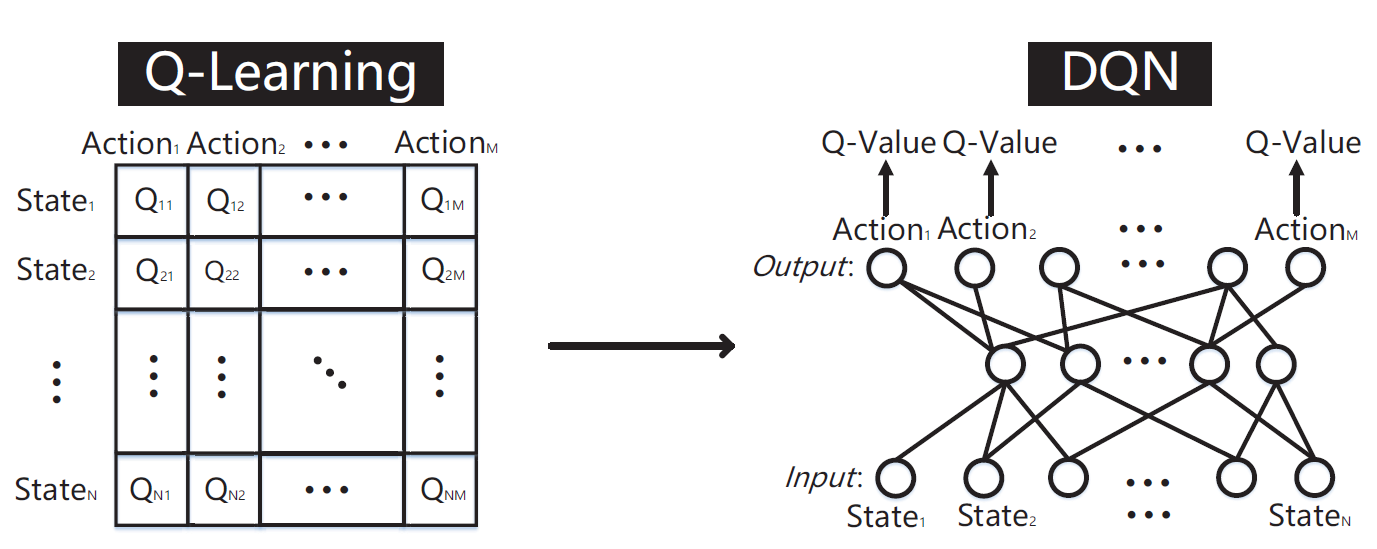
\includegraphics[scale=0.4]{./Figure/QvsDQN.png}
  \caption{Difference between Q-learning and DQN \cite{zhang2019end}}
  \label{fig:QvsDQN}
\end{figure}

\section{Previous Research and Motivation}
\label{sec:motivation}
This paper includes three motivations. First motivation explains the reason to employ RL for Forex trading. 

Before employing RL for finance in earnest, the papers that applied machine learning tended to focus on predicting the future. For example, Arash's survey \cite{bahrammirzaee2010} showed that many papers about trading were related to prediction.

The weakness in the predictive approach is to ignore the option to wait. For example, when a trader cannot be sure the direction of the exchange rate, the best strategy should be to wait without bringing any profit and any loss. However, the predictive approach completely disregards that option.

On the other hand, RL allows the agent to consider waiting as part of actions. This is the reason to employ RL in my research.

Second motivation is utilization of DQN. In terms of RL modeling, Forex trading can be characterized by the continuous of the state while the action is discrete. This is because, in most cases, the state definition includes the exchange rate history which is continuous. On the other hand, the action can be defined as discrete like the position transition in Figure \ref{fig:pos_trans}.

As mentioned in Section \ref{sec:DQL}, DQN is suitable for the modeling where the state and the action are defined as continuous and discrete respectively. This is why this research employs DQN.

The third motivation is to confirm the effect of metrics. Among Forex technical analysis, many metrics are utilized. This research focuses on simple moving average (MA) which is one of the most basic metrics in the analysis \cite{analysisMA}. The experiment verifies whether MA as state element of RL improves the performance of the agent.

\chapter{Method and Algorithm}
\label{sec:method_algo}
\section{Overview}
This paper employs RL as Figure \ref{fig:methodOverview}. To maximize the reward, the Q-values are calculated as the right side of Figure \ref{fig:QvsDQN} using DQN.
\begin{figure}[htbp]
  \centering
  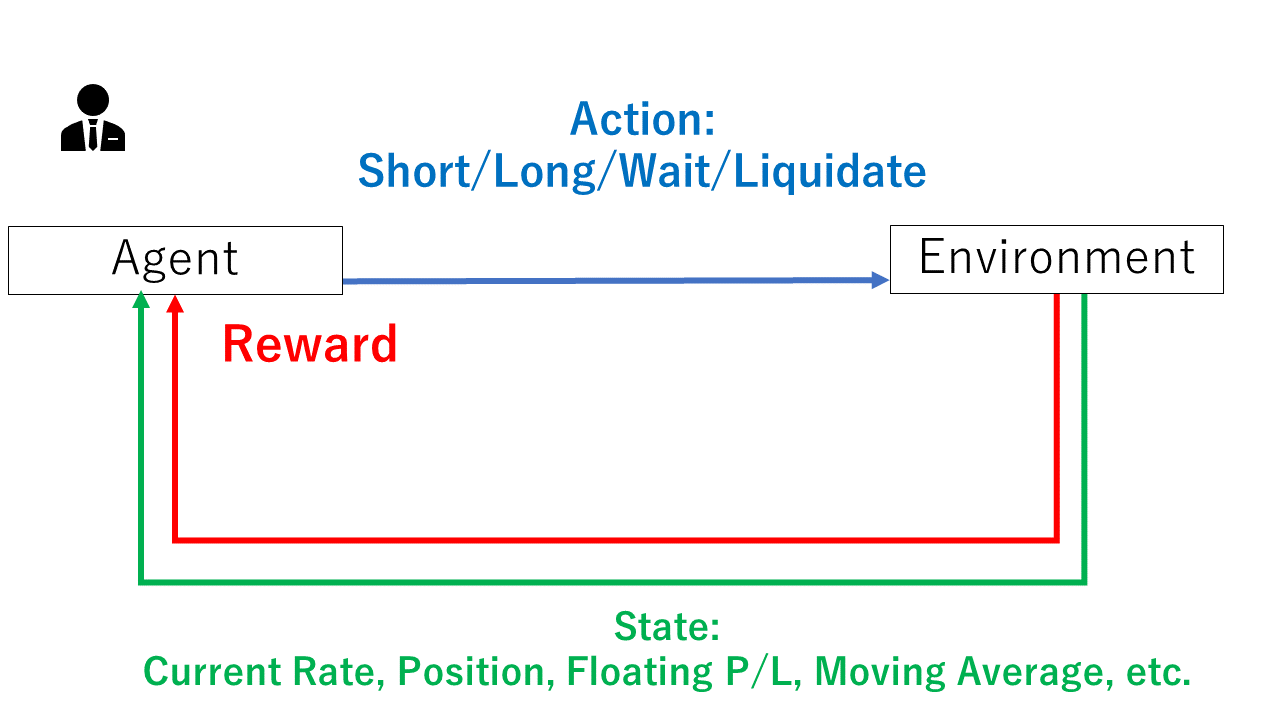
\includegraphics[scale=0.4]{./Figure/method_overview.png}
  \caption{RL for Forex trading}
  \label{fig:methodOverview}
\end{figure}

\section{State}
\label{sec:state}
The {\it state element} is defined as Equation (\ref{eq:state-el}) 
\begin{equation}
  \label{eq:state-el}
\mbox{ \boldmath{ $ S_{t} $}} = (cu_{t}, pos, ma1_{t}, ma2_{t}, ma3_{t}, ma4_{t}, ma5_{t}, fpl_{t}, pos\_rate).
\end{equation}
The subscript $t$ means {\it time step}, and the same applies hereafter. The $t$ starts with 120 to calculate the moving average $ma1_{t}$.

The $cu_{t}$ means {\it current exchange rate}.

Denoted as $pos$, the (\ref{eq:pos}) defines {\it current position} as
\begin{equation}
  \label{eq:pos}
   pos \in \{ SQUARE, SHORT, LONG \},
\end{equation}
where the agent is in.

Equation (\ref{eq:ma}) means {\it moving averages}:
\begin{equation}
  \label{eq:ma}
  \begin{array}{l}
    ma1_{t} = \frac{1}{120} \displaystyle \sum_{i=t-120}^{t} p_i, \\
    ma2_{t} = \frac{1}{80} \displaystyle \sum_{i=t-80}^{t} p_i,   \\
    ma3_{t} = \frac{1}{50} \displaystyle \sum_{i=t-50}^{t} p_i,   \\
    ma4_{t} = \frac{1}{30} \displaystyle \sum_{i=t-30}^{t} p_i,   \\
    ma5_{t} = \frac{1}{20} \displaystyle \sum_{i=t-20}^{t} p_i.   \\
  \end{array}
\end{equation}
The $p_i$ means the exchange rate (price) at the time step $i$.

Equation (\ref{eq:fpl-def}) means {\it floating P/L} which corresponds to Section \ref{sec:Forex}:
\begin{equation}
  \label{eq:fpl-def}
  fpl_{t} =
  \left\{
    \begin{array}{l}
      cu_{t} - pos\_rate  \ (pos=LONG)\\
      pos\_rate - cu_{t}  \ (pos=SHORT)\\
      0 \ (otherwise)
    \end{array}
  \right..
\end{equation}

The $pos\_rate$ means the {\it exchange rate when taking the position}. For example, the $pos\_rate=112.55$ means that the 1 dollar had equaled 112.55 yen when the agent had taken the long or the short position. If the agent is in the square, the $pos\_rate$ becomes zero.

\section{Deviation of Exchange Rate Data}
\label{sec:devEx}
In fact, all data of the exchange rate is normalized as Equation \ref{eq:normlize} 
\begin{equation}
  \label{eq:normlize}
  p_{t} = d_{t} - \frac{1}{N} \sum_{i=1}^{N} d_i,
\end{equation}
where the $N$ means the time period of the entire data history. The $d_t$ means original data of the dataset in Section \ref{sec:dataset}. The time period $N$ depends on the number of the data in Table \ref{tb:dataset}.

The normalization narrows the range between maximum and minimum in the state space to reduce computational complexity.

\section{Action}
\label{sec:action}
The {\it action set} $\mathcal{A}$ is defined as Equation (\ref{eq:action-set}):
\begin{equation}
  \label{eq:action-set}
  \begin{array}{l}
   \mathcal{A}( \mbox{\boldmath{$ pos=SQUARE $}} )=\{ WAIT, SHORT, LONG \} \\
   \mathcal{A}( \mbox{\boldmath{$ pos=ohterwise $}} )=\{ WAIT, LIQUIDATE \}.
  \end{array}
\end{equation}
Equation (\ref{eq:action-set}) corresponds to the position transition as Figure \ref{fig:pos_trans}.

The (\ref{eq:action-element}) shows each {\it action element} $A_{t}$ belongs to the action set. Each action element $A_{t}$ means taken action at time $t$.
\begin{equation}
  \label{eq:action-element}
  A_{t} \in \mathcal{A}( \mbox{\boldmath{$ pos $}} )
\end{equation}

\section{Action Modification}
\label{sec:actMod}
Despite Equation \ref{eq:action-set}, the agent may take wrong action. For example, he may liquidate wrongly even when he is in the square. This is because the agent must learn the position transition of Figure \ref{fig:pos_trans} although the transition is deterministic.

Therefore, the RL system is implemented to replace a wrong action with the {\it wait} action as below.
\begin{itemize}
  \item In Square: the agent wrongly {\it liquidates} $\Longrightarrow$  {\it wait} action
  \item In Short of Long position: the agent wrongly takes {\it long} or {\it short} position $\Longrightarrow$  {\it wait} action
\end{itemize}

In addition, the RL system forces the agent to liquidate his position forcefully when one episode finishes. If the system does not, the agent can keep waiting to avoid losses in any case even if he takes a long or short position.

\section{Episode}
The final time step $T$ of one episode is defined as Equation (\ref{eq:T-period}) 
\begin{equation}
  \label{eq:T-period}
  T = 1200.
\end{equation}

One {\it episode} is defined as the (\ref{eq:one-episode})  
\begin{equation}
  \label{eq:one-episode}
  \mbox{ \boldmath{ $ S_{0} $}}, A_{0}, \quad R_{1}, \mbox{ \boldmath{ $ S_{1} $}}, A_{1}, \quad R_{2}, \mbox{ \boldmath{ $ S_{2} $}}, A_{2}, \quad ...,\quad  R_{T-1}, \mbox{ \boldmath{ $ S_{T-1} $}}, A_{T-1}, \quad R_{T}, \mbox{ \boldmath{ $ S_{T} $}},
\end{equation}

One {\it step} is defined as Equation (\ref{eq:one-step})
\begin{equation}
  \label{eq:one-step}
  step = 
  \left\{
    \begin{array}{l}
      \mbox{ \boldmath{ $ S_{t} $}}, A_{t}       \qquad (t=0)\\
      R_{t}, \mbox{ \boldmath{ $ S_{t} $}}, A_{t} \ (otherwise)\\
    \end{array}
  \right.,
\end{equation}


\section{P/L and Reward}
\label{sec:pl_reward}
Equation (\ref{eq:pl-calc}) means profit and loss (P/L) which corresponds to Section \ref{sec:Forex}:
\begin{equation}
  \label{eq:pl-calc}
  profit =
  \left\{
    \begin{array}{l}
      (cu_{t} - pos\_rate) \times 10000  \ (pos=LONG \ \land \ a= LIQUIDATE)\\
      (pos\_rate - cu_{t}) \times 10000  \ (pos=SHORT\ \land \ a= LIQUIDATE)\\
      0                          \ (otherwise)\\
    \end{array}
  \right.,
\end{equation}
where $\times 10000$ is leverage to amplify P/L. The negative profit means losses.

Note that the $cu_{t}$ is the current exchange rate of time $t$, not $t+1$ of cover deal in Section \ref{sec:Forex}. It is simplification in order to make implementation easy.

In this research, the {\it reward} is defined as same as the profit. Note that the leverage enables the agent to learn because the normalization in Section \ref{sec:devEx} makes the reward without the leverage close to zero.

\section{DQN}
\label{sec:DQN}
As agent of RL, this research utilizes DQN \cite{mnih2013playing} where the policy is Boltzmann Q Policy, or soft-max policy.

The neural network is constructed with Keras as below:
\begin{lstlisting}[caption=Neural network structure with Keras, label=list:network]
  Layer (type)                 Output Shape              Param #   
  =================================================================
  flatten_1 (Flatten)          (None, 9)                 0         
  _________________________________________________________________
  dense_1 (Dense)              (None, 16)                160       
  _________________________________________________________________
  activation_1 (Activation)    (None, 16)                0         
  _________________________________________________________________
  dense_2 (Dense)              (None, 16)                272       
  _________________________________________________________________
  activation_2 (Activation)    (None, 16)                0         
  _________________________________________________________________
  dense_3 (Dense)              (None, 16)                272       
  _________________________________________________________________
  activation_3 (Activation)    (None, 16)                0         
  _________________________________________________________________
  dense_4 (Dense)              (None, 4)                 68        
  _________________________________________________________________
  activation_4 (Activation)    (None, 4)                 0         
  =================================================================
  Total params: 772
  Trainable params: 772
  Non-trainable params: 0
\end{lstlisting}

In Listing \ref{list:network}, the flatten\_1 layer is the input layer which takes the state elements as Equation \ref{eq:state-el}. The activation\_1, activation\_2, and activation\_3 layers utilize ReLU (Rectified Linear Unit) activation \cite{relu}, and the activation\_4 layer uses linear activation \cite{linear}. The dense\_1, dense\_2, dense\_3 and dense\_4 layers are densely-connected (fully-connected) neural network layers \cite{dense}. The activation\_4 corresponds to the output layer on the right side of Figure \ref{fig:QvsDQN} to decide to take an action as WAIT, SHORT, LONG or LIQUIDATE.

\chapter{Experiment}
\label{sec:experiment}
The agent is trained based on Section \ref{sec:method_algo} by 50,000 steps trading on the testing dataset which mostly equals 47 episodes. Each training episode consists of same data. After that, the agent is tested by trading of one episode on nine testing datasets. Note that each testing dataset make each environment interact with the agent exactly the same every episode. This is why testing consists of one episode.

To confirm the effect of MA as metrics, the training and nine testing vary the number of MA from zero to five. For example, when the number of MA is four which is denoted as MA4, the MA elements are changed as Equation \ref{eq:ma4}. When the number of MA is three which is denoted as MA3, the MA elements are changed as Equation \ref{eq:ma3}, and so on. 

\begin{equation}
  \label{eq:ma4}
  \begin{array}{l}
    ma1_{t} = \frac{1}{120} \displaystyle \sum_{i=t-120}^{t} p_i, \\
    ma2_{t} = \frac{1}{80} \displaystyle \sum_{i=t-80}^{t} p_i,   \\
    ma3_{t} = \frac{1}{50} \displaystyle \sum_{i=t-50}^{t} p_i,   \\
    ma4_{t} = \frac{1}{30} \displaystyle \sum_{i=t-30}^{t} p_i,   \\
    ma5_{t} = 0   \\
  \end{array}
\end{equation}

\begin{equation}
  \label{eq:ma3}
  \begin{array}{l}
    ma1_{t} = \frac{1}{120} \displaystyle \sum_{i=t-120}^{t} p_i, \\
    ma2_{t} = \frac{1}{80} \displaystyle \sum_{i=t-80}^{t} p_i,   \\
    ma3_{t} = \frac{1}{50} \displaystyle \sum_{i=t-50}^{t} p_i,   \\
    ma4_{t} = 0,   \\
    ma5_{t} = 0   \\
  \end{array}
\end{equation}

\section{Dataset}
\label{sec:dataset}
The dataset consists of the USD/JPY (US Dollar vs. Japanese Yen) exchange rate where the candlestick range is five minutes. It is comprised of the training dataset and nine testing datasets as Table \ref{tb:dataset} shows. Note that the trained/tested data are not the entire ones but 1200 ones that correspond to Equation \ref{eq:T-period}, which is listed as Trained/Tested Data Period column on Table \ref{tb:dataset}.

\begin{table}[htb]
  \centering
  \caption{Dataset of training and testing}
  \label{tb:dataset}
  \begin{tabular}{|c|c|c|c|}
  \hline
    Dataset Name & Period (Day.Month.Year, GMT)  & Number of Data & Trained/Tested Data Period \\
  \hline
    Train        & 01.01.2004 - 09.01.2004  & 1908           & 01.01.2004 - 07.01.2004  \\
    Test 1       & 11.01.2004 - 20.01.2004  & 2040           & 11.01.2004 - 16.01.2004  \\
    Test 2       & 01.02.2004 - 10.02.2004  & 2040           & 01.02.2004 - 06.02.2004  \\
    Test 3       & 20.06.2004 - 30.06.2004  & 2340           & 20.06.2004 - 25.06.2004  \\
    Test 4       & 02.01.2005 - 10.01.2005  & 1752           & 02.01.2005 - 07.01.2005  \\
    Test 5       & 01.01.2007 - 10.01.2007  & 2302           & 01.01.2007 - 05.01.2007  \\
    Test 6       & 01.01.2009 - 09.01.2009  & 1992           & 01.01.2009 - 07.01.2009  \\
    Test 7       & 02.01.2011 - 10.01.2011  & 1752           & 02.01.2011 - 07.01.2011  \\
    Test 8       & 01.01.2014 - 10.01.2014  & 2016           & 01.01.2014 - 08.01.2014  \\
    Test 9       & 01.01.2019 - 10.01.2019  & 2040           & 01.01.2019 - 08.01.2019  \\
  \hline
  \end{tabular}
\end{table}

\section{Evaluation Method}
\label{sec:evaluation}
The evaluation method consists of two parts: accumulated reward and waiting ratio. 

The first evaluation method is the {\it accumulated reward} which is defined as total rewards per one episode. It means the performance of agent's Forex trading. Note that the accumulated reward is equivalent to total P/L per one episode due to the definition of Section \ref{sec:pl_reward}.

The second evaluation method is the {\it waiting ratio} defined as Equation \ref{eq:waiting_def}
\begin{equation}
  \label{eq:waiting_def}
  \begin{array}{l}
    waiting \ ratio = \frac{the \ number \ of \ waiting \ in \ one \ episode}{the \ number \ of \ total \ actions \ in \ one \ episode}. \\
  \end{array}
\end{equation}
As mentioned in Section \ref{sec:motivation}, when a trader cannot be sure the direction of the exchange rate, he should wait. The waiting ratio shows whether RL realizes this strategy. The further the period of testing dataset is from the training period, the more the waiting ratio should increase.


\section{Details}
For details about source code and dataset, see the GitHub repository \cite{src}.

\chapter{Result}
\label{sec:result}
\section{Accumulated Reward}
Figure \ref{fig:acRewardTrain} shows the accumulated reward of each MA for each training episode. It suggests that the agent cannot learn how to make a profit because even the second half of the episodes show mostly negative rewards, as well as Table \ref{tb:acRewardTrain10} shows. In addition, the number of MA seems to have little impact on the reward in the training.


\begin{figure}[htbp]
  \centering
  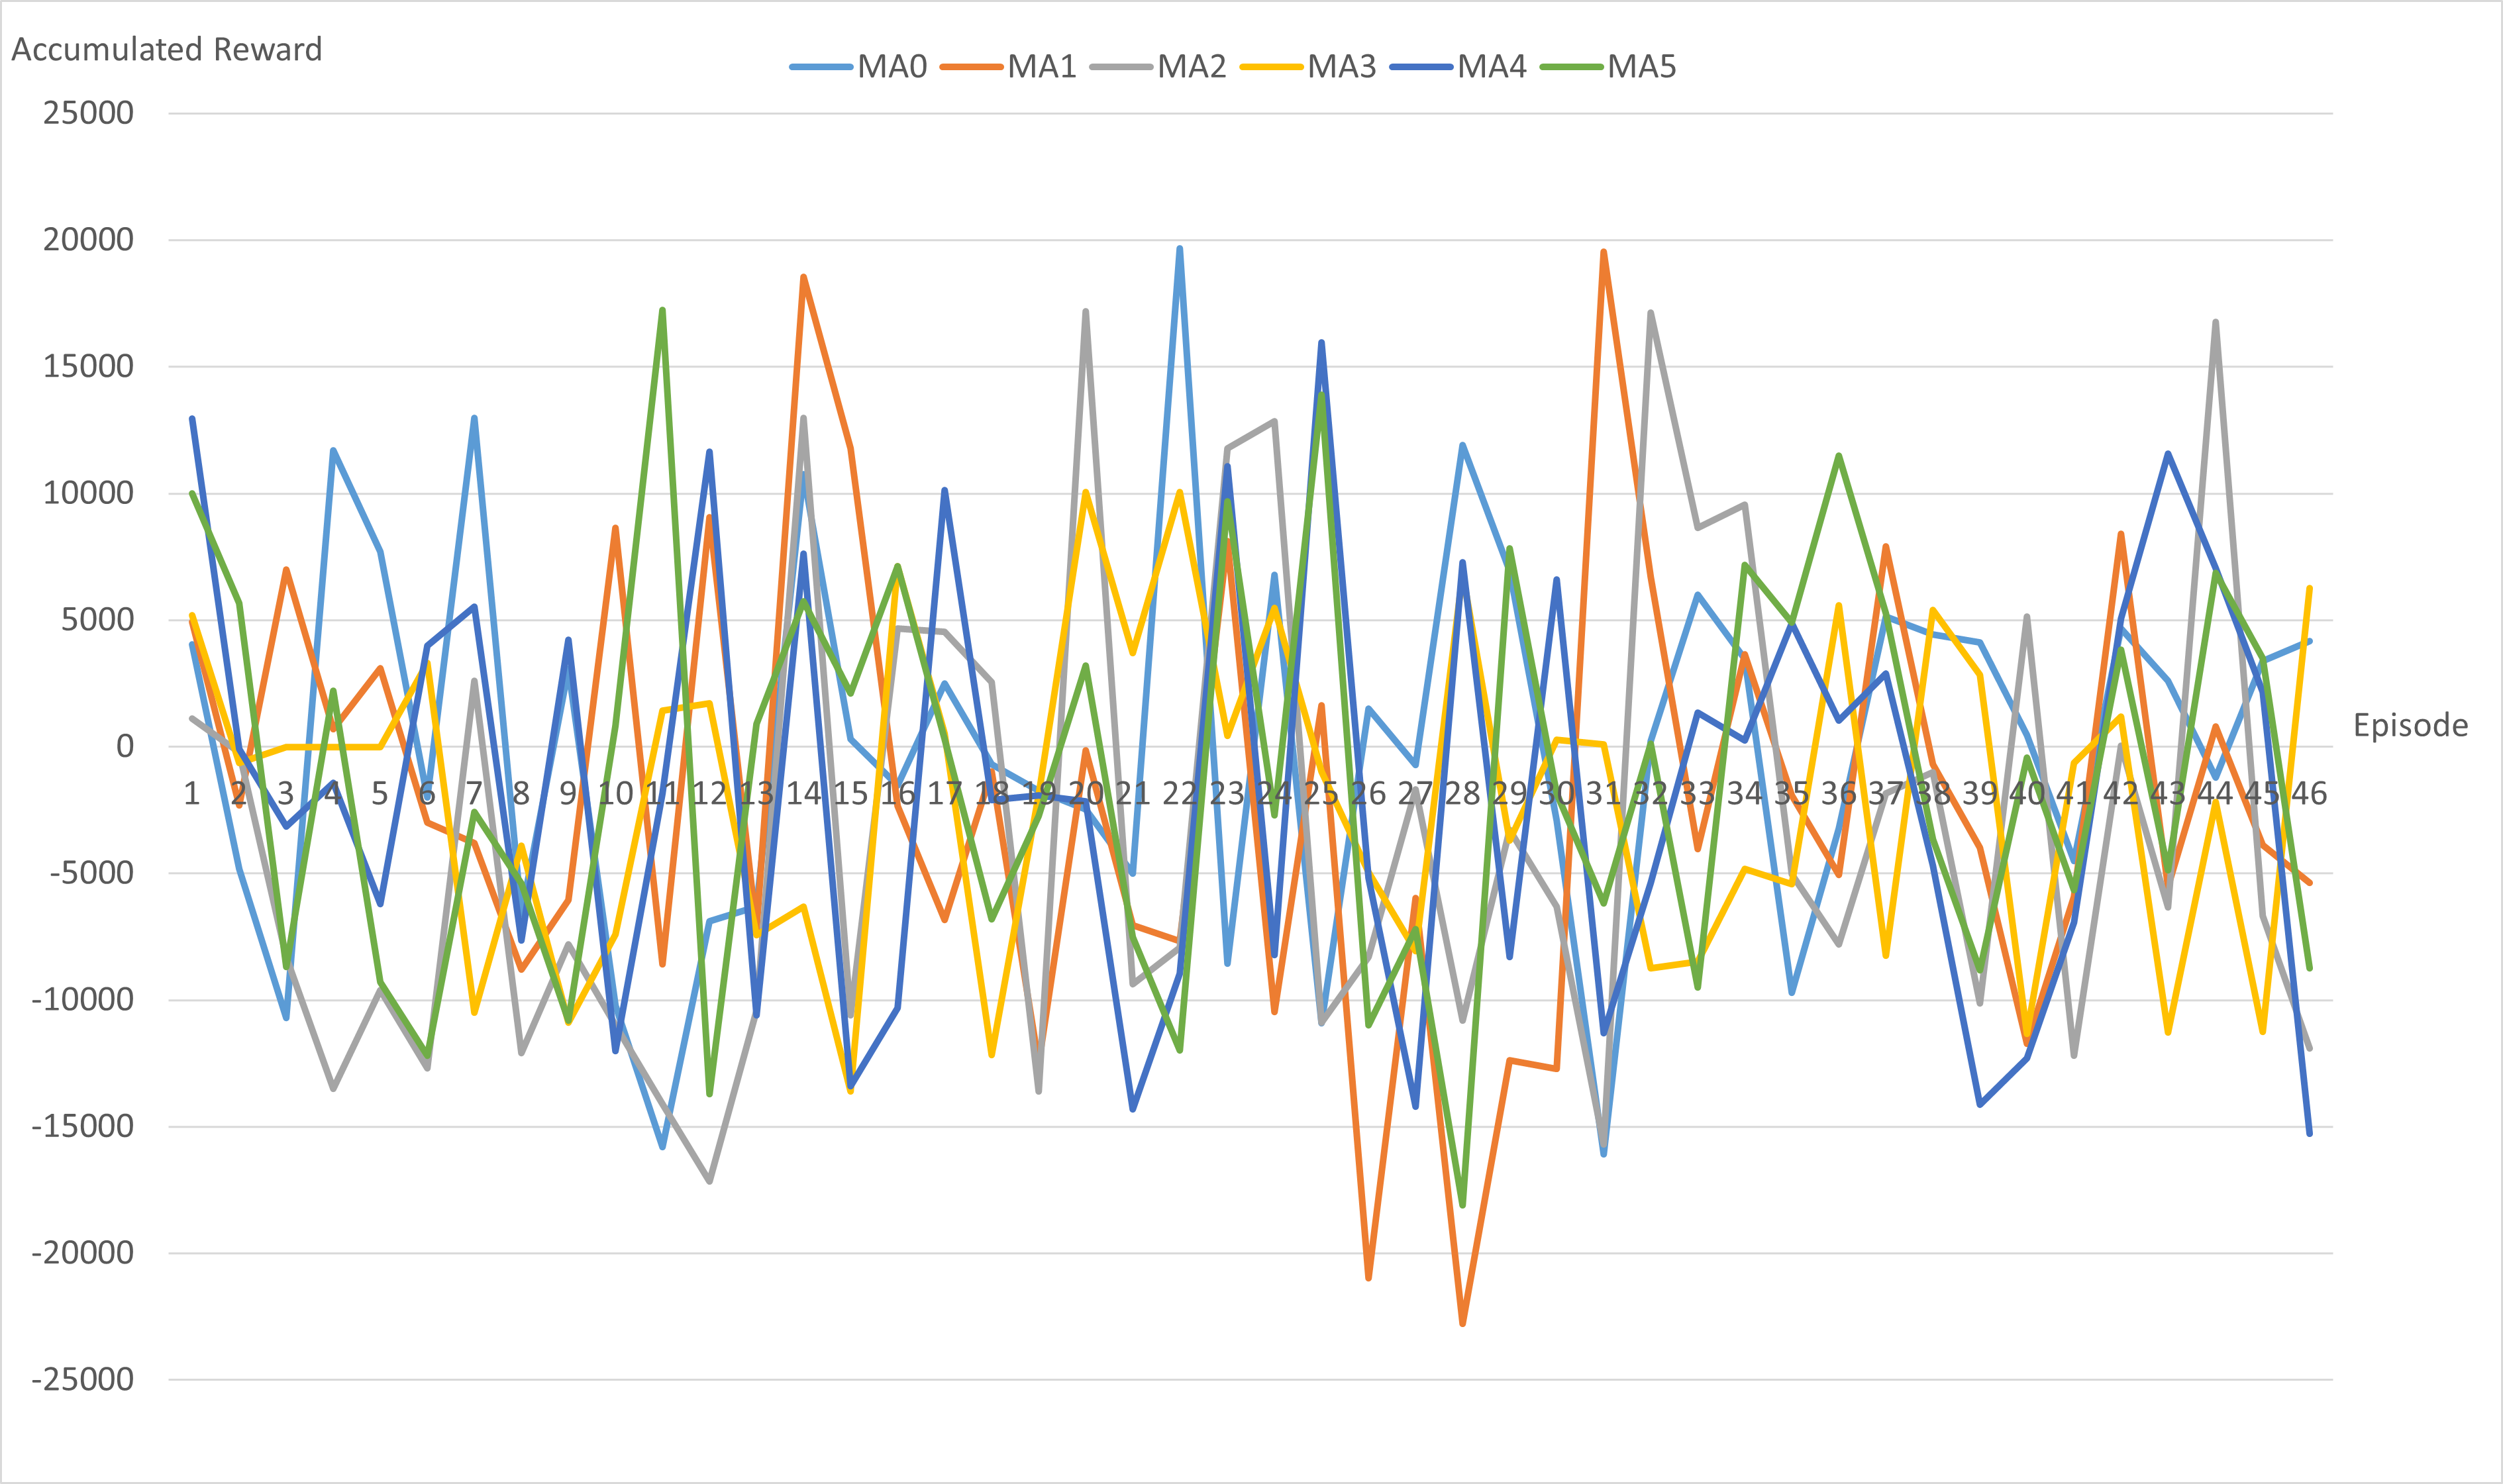
\includegraphics[scale=0.5]{./Figure/acRewardTrain.png}
  \caption{Accumulated reward in training for the number of moving average (MA)}
  \label{fig:acRewardTrain}
\end{figure}

\begin{table}[htb]
  % Source: The row "last 10 avg." of rewardVStrain_formatted.xlsx
  \centering
  \caption{The average of accumulated reward in the last ten trainings for each MA}
  \label{tb:acRewardTrain10}
  \begin{tabular}{|c|c|c|c|c|c|}
  \hline
    MA0  & MA1   & MA2    & MA3   & MA4    & MA5   \\
  \hline
    954  & -2748 & -2169  & -2785 & -2123  & -1205 \\
  \hline
  \end{tabular}
\end{table}

The same is true for Figure \ref{fig:acRewardTest}. Most rewards of the tests are negative, and the figure suggests that the number of MA could not improve the trading performance since each MA shows similar accumulated rewards. If the number of MA had some sort of impact on the performance, each MA would show the different accumulated reward.

As a result, it is concluded that MA may be invalid metrics for DQL of Forex trading.
\begin{figure}[htbp]
  \centering
  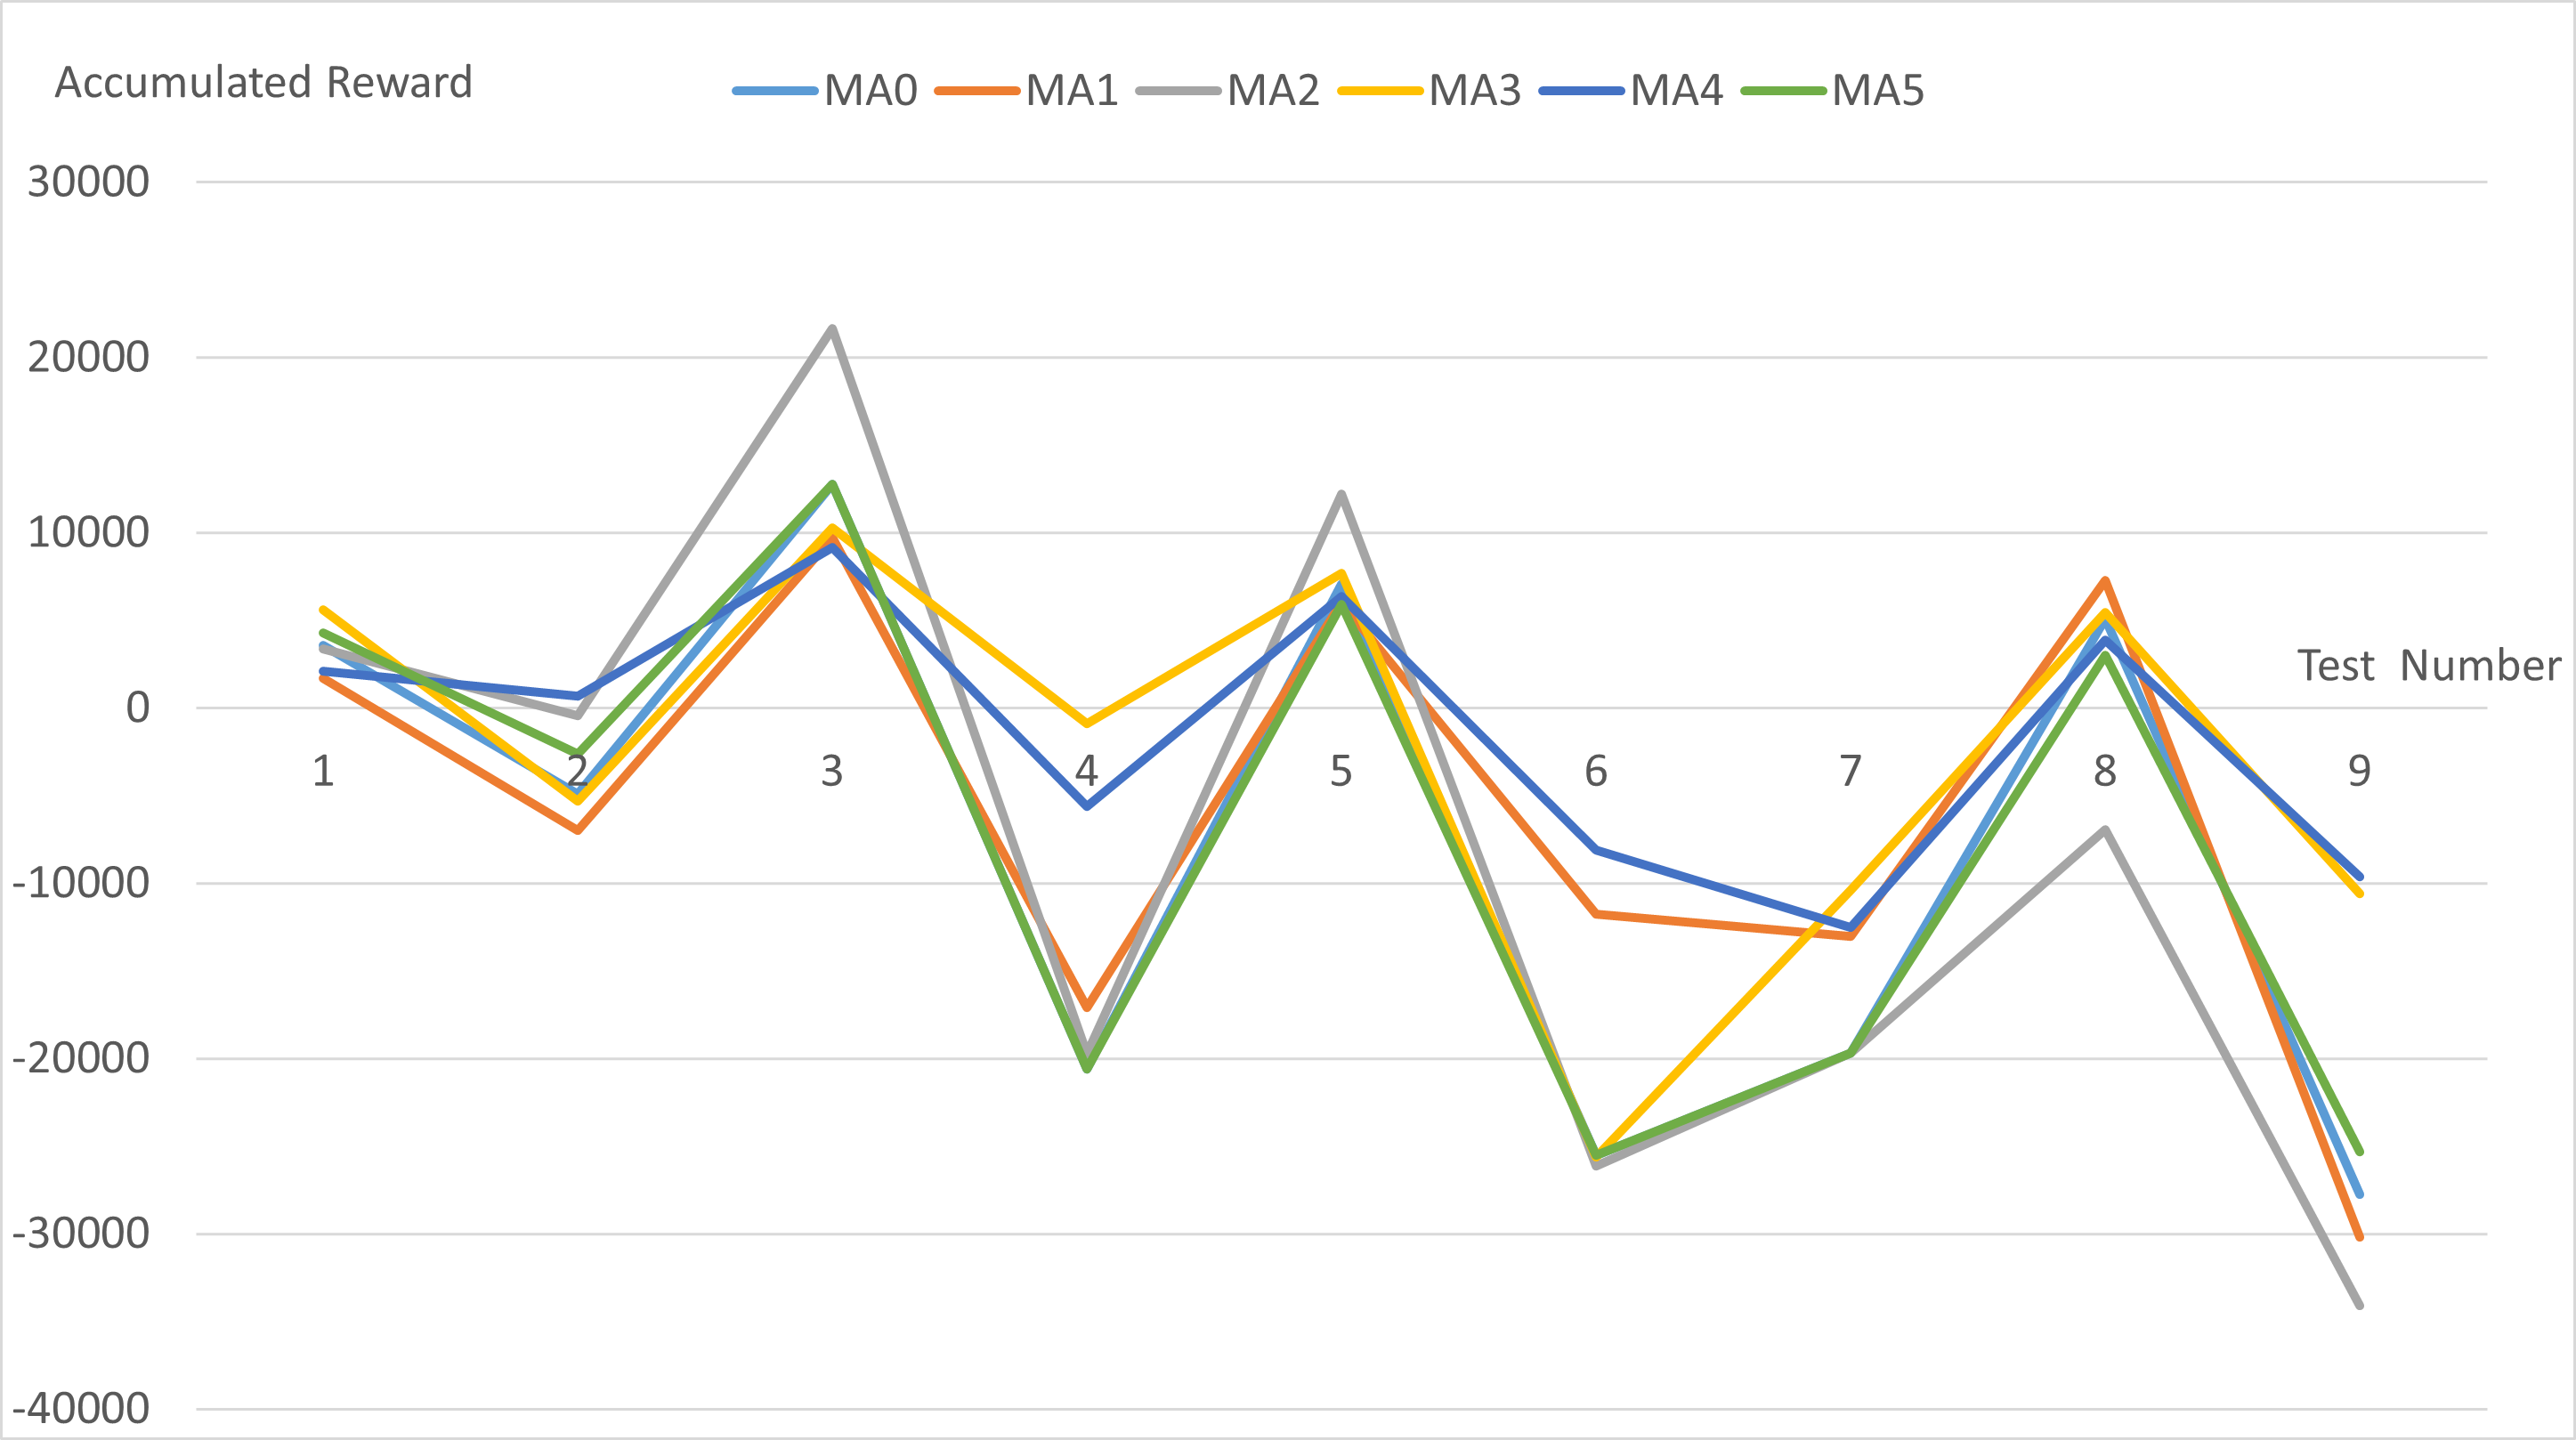
\includegraphics[scale=0.5]{./Figure/acRewardTest.png}
  \caption{Accumulated reward in testing for the number of MA}
  \label{fig:acRewardTest}
\end{figure}


\section{Waiting Ratio}
\label{sec:waitingRatioResult}
Figure \ref{fig:waitingTrain} is the chart of the waiting ratio for each MA in the training episodes. It suggests that the waiting ratios of any number of MA tend to converge to the range of 70\% to 75\% as well as Figure \ref{fig:waitingTrainAvg} shows. 

From Figure \ref{fig:ma0waitingReward} to Figure \ref{fig:ma5waitingReward}, these figures indicate that the range of 70\% to 75\% is the boundary whether the loss absolutely occurs or not: the right sides of the range in the figures show that most data points are negative accumulated rewards.

RL is presumed to help to avoid losses in Forex trading. As explained in the previous section, it was difficult for the agent to get profit with MA metrics, therefore the agent seemingly focuses on avoiding losses. 

\begin{figure}[htbp]
  \centering
  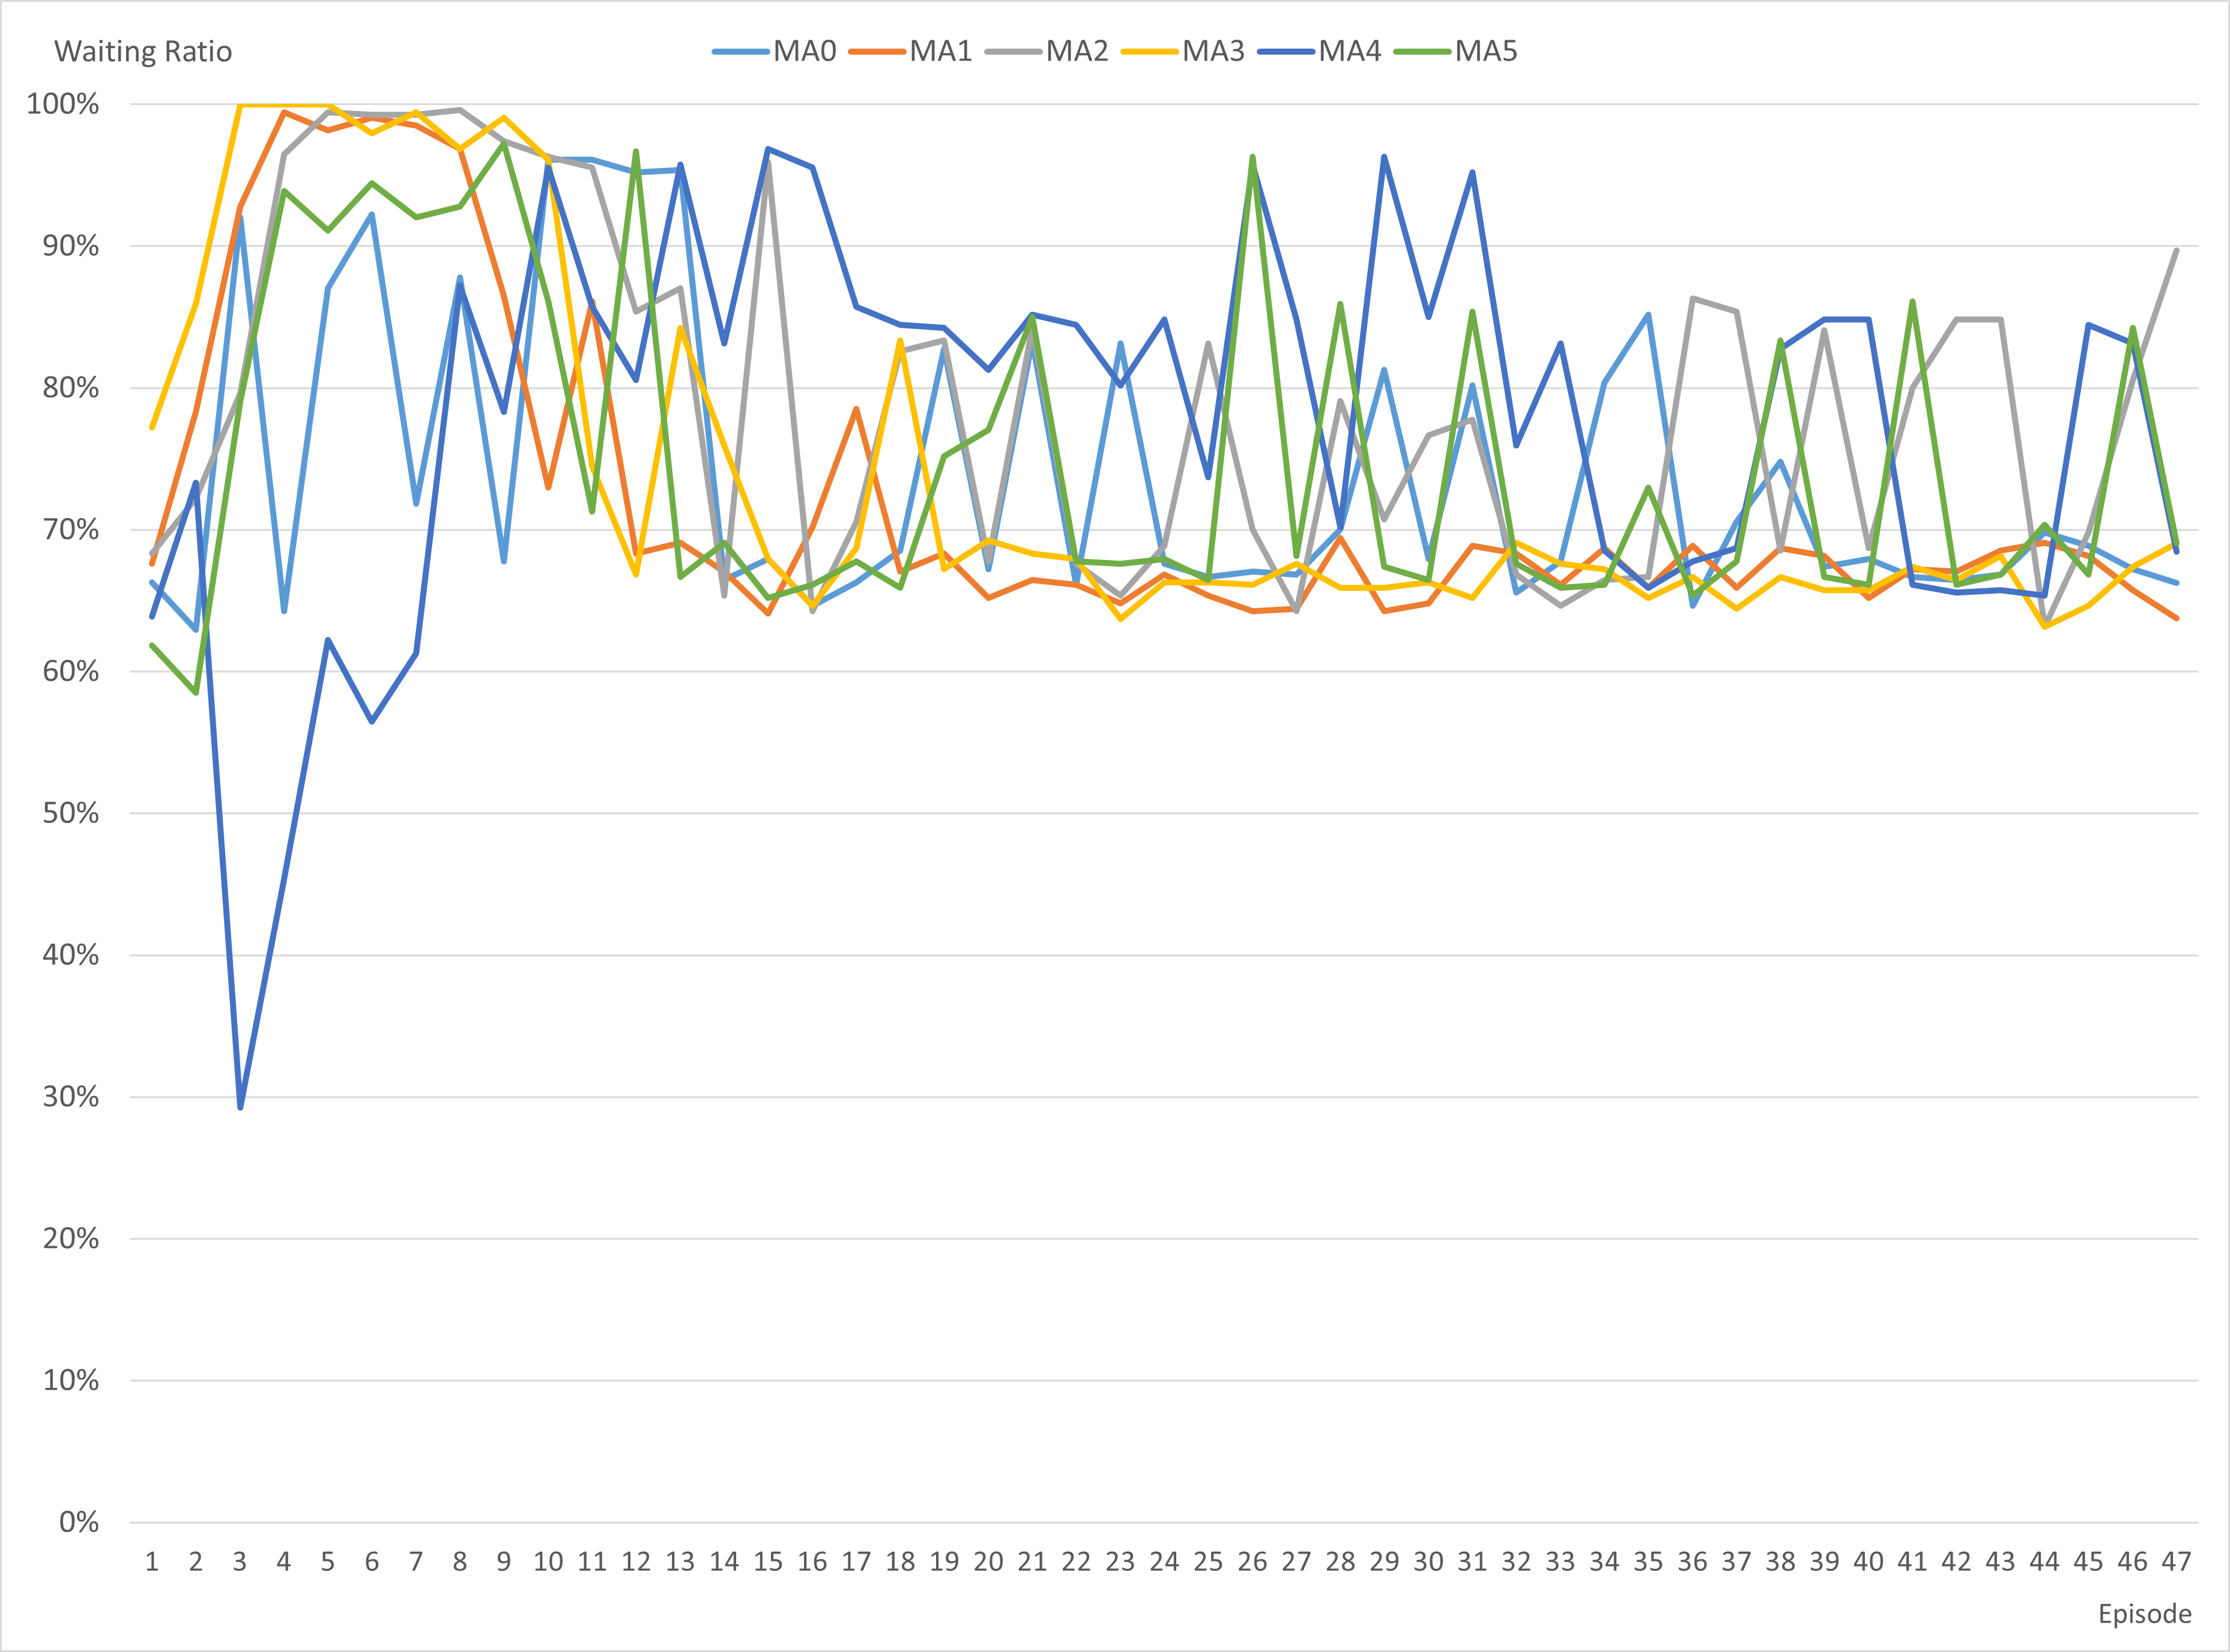
\includegraphics[scale=0.5]{./Figure/waitingTrain.png}
  \caption{Waiting ratio in training for the number of MA}
  \label{fig:waitingTrain}
\end{figure}

\begin{figure}[htbp]
  \centering
  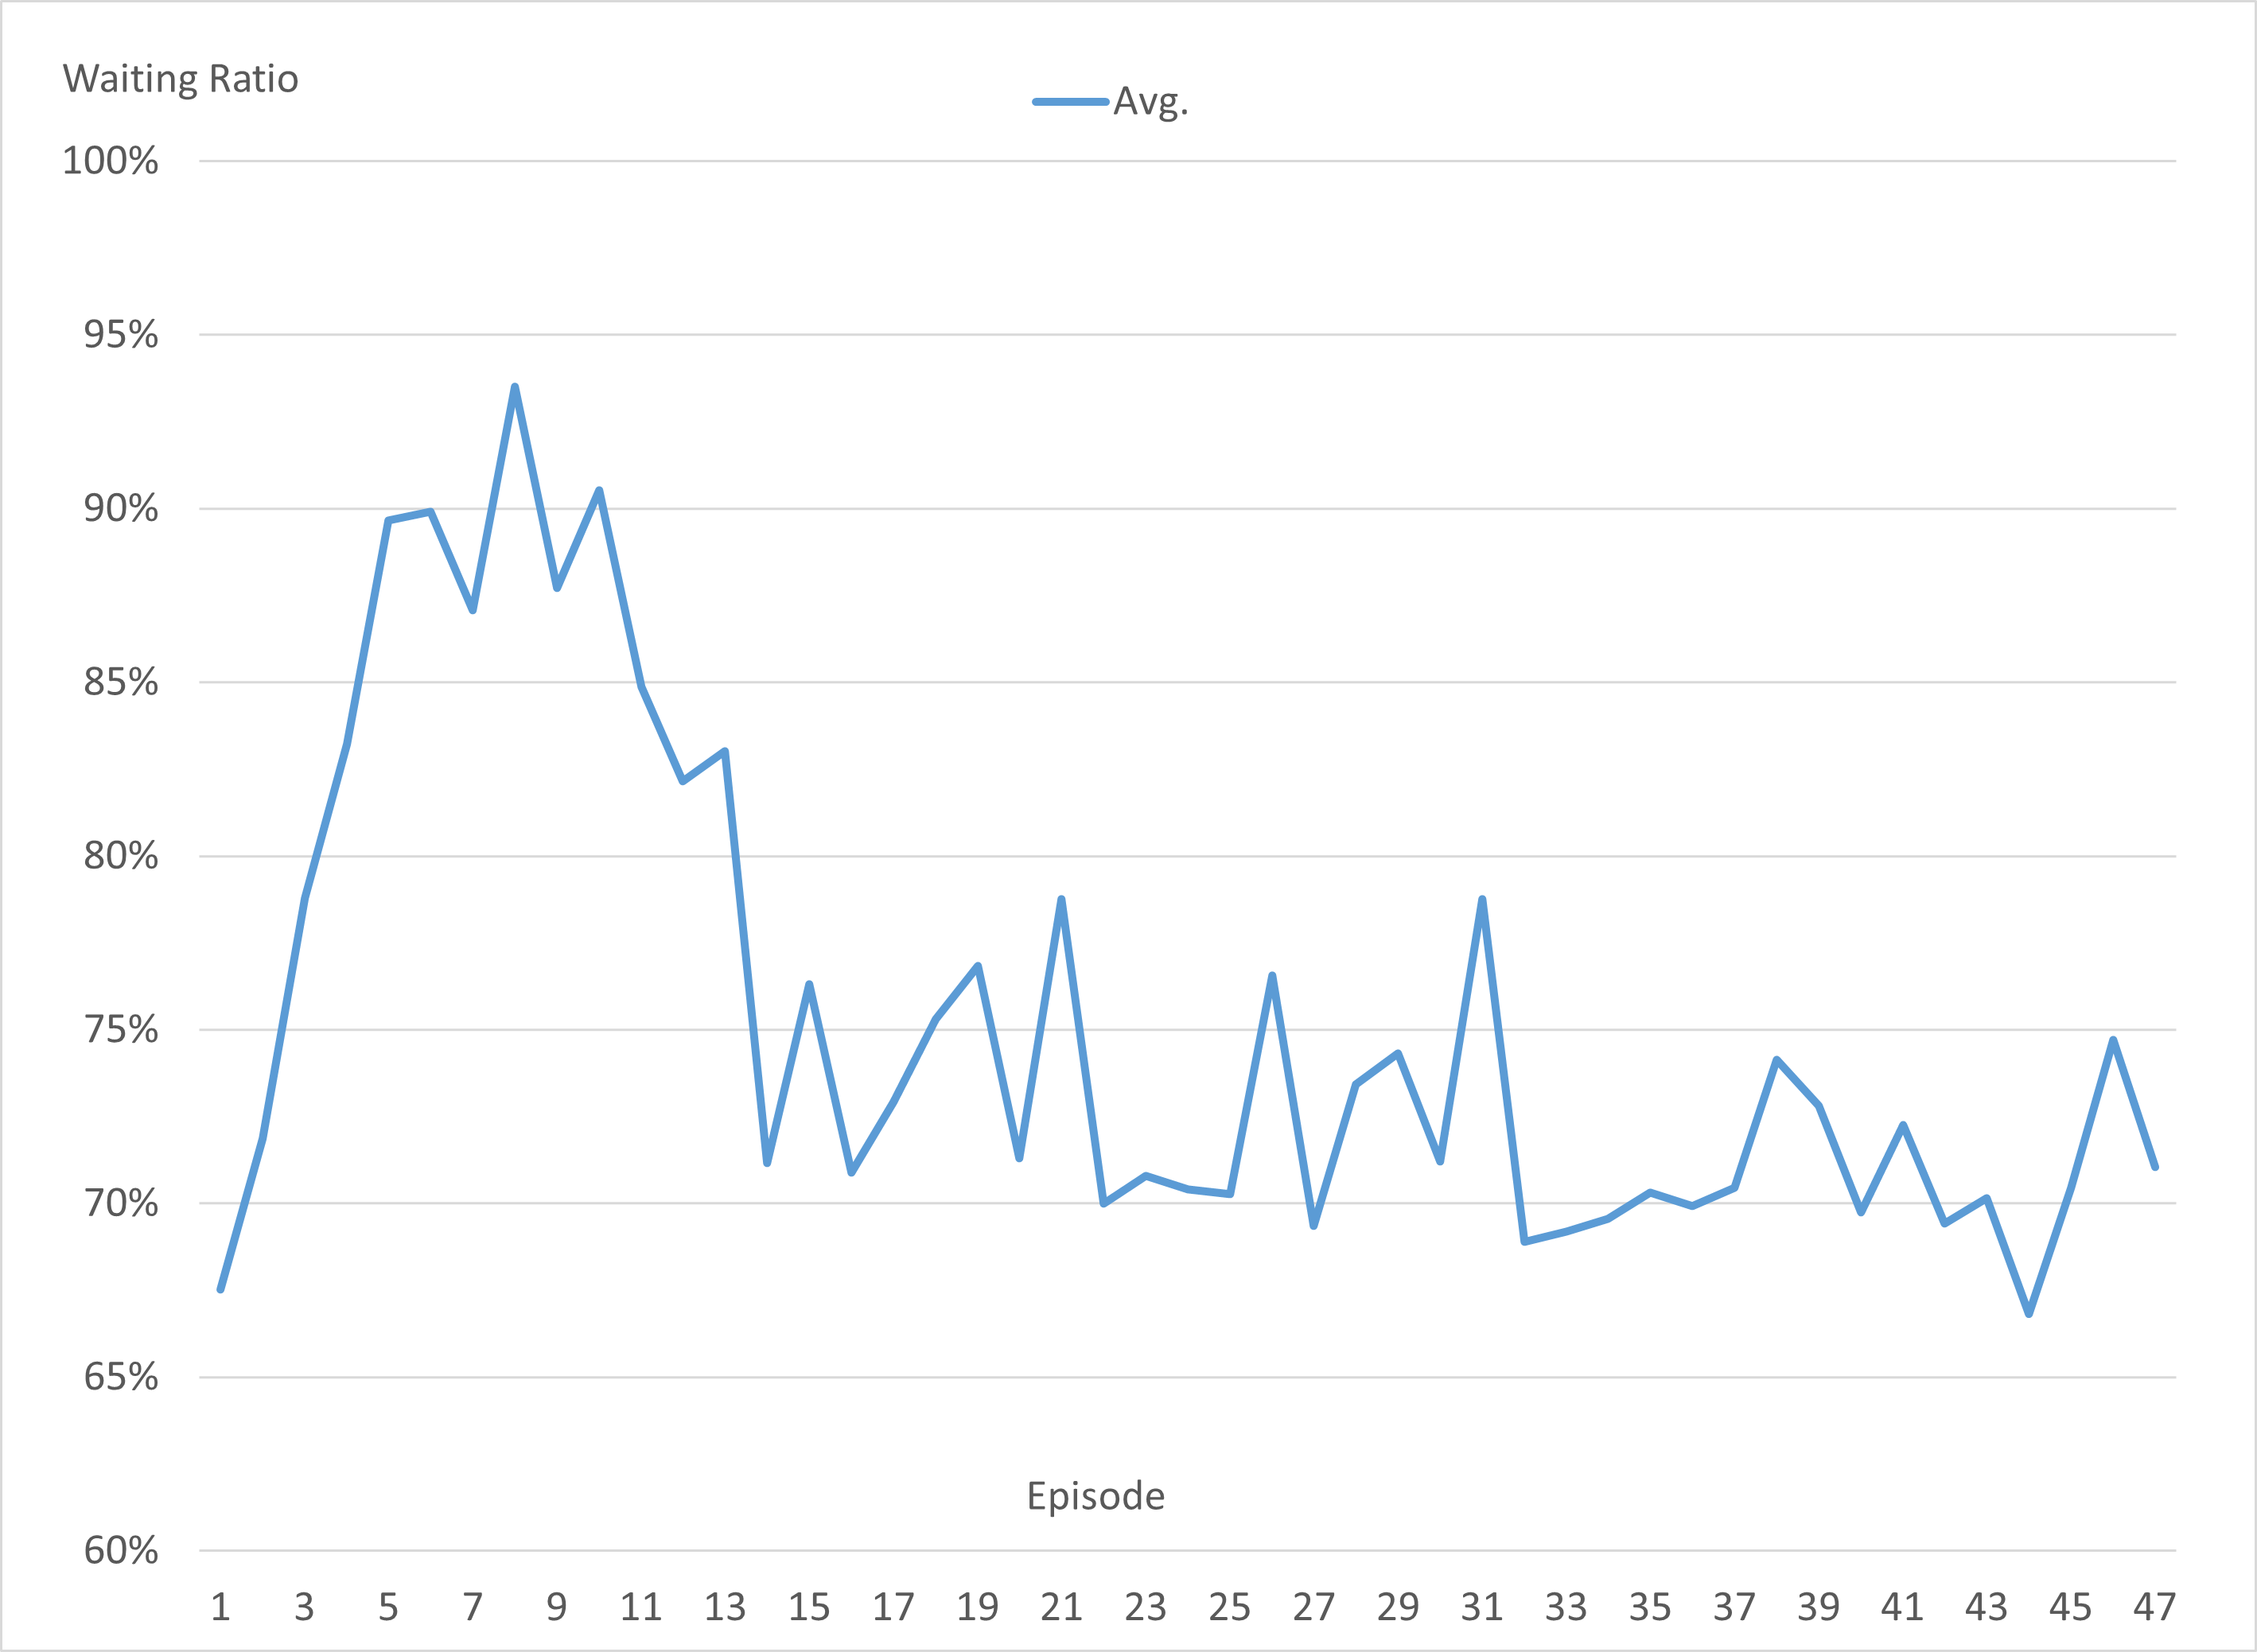
\includegraphics[scale=0.5]{./Figure/waitingTrainAvg.png}
  \caption{Average of waiting ratio in testing for the number of MA}
  \label{fig:waitingTrainAvg}
\end{figure}

\begin{figure}[htbp]
  \centering
  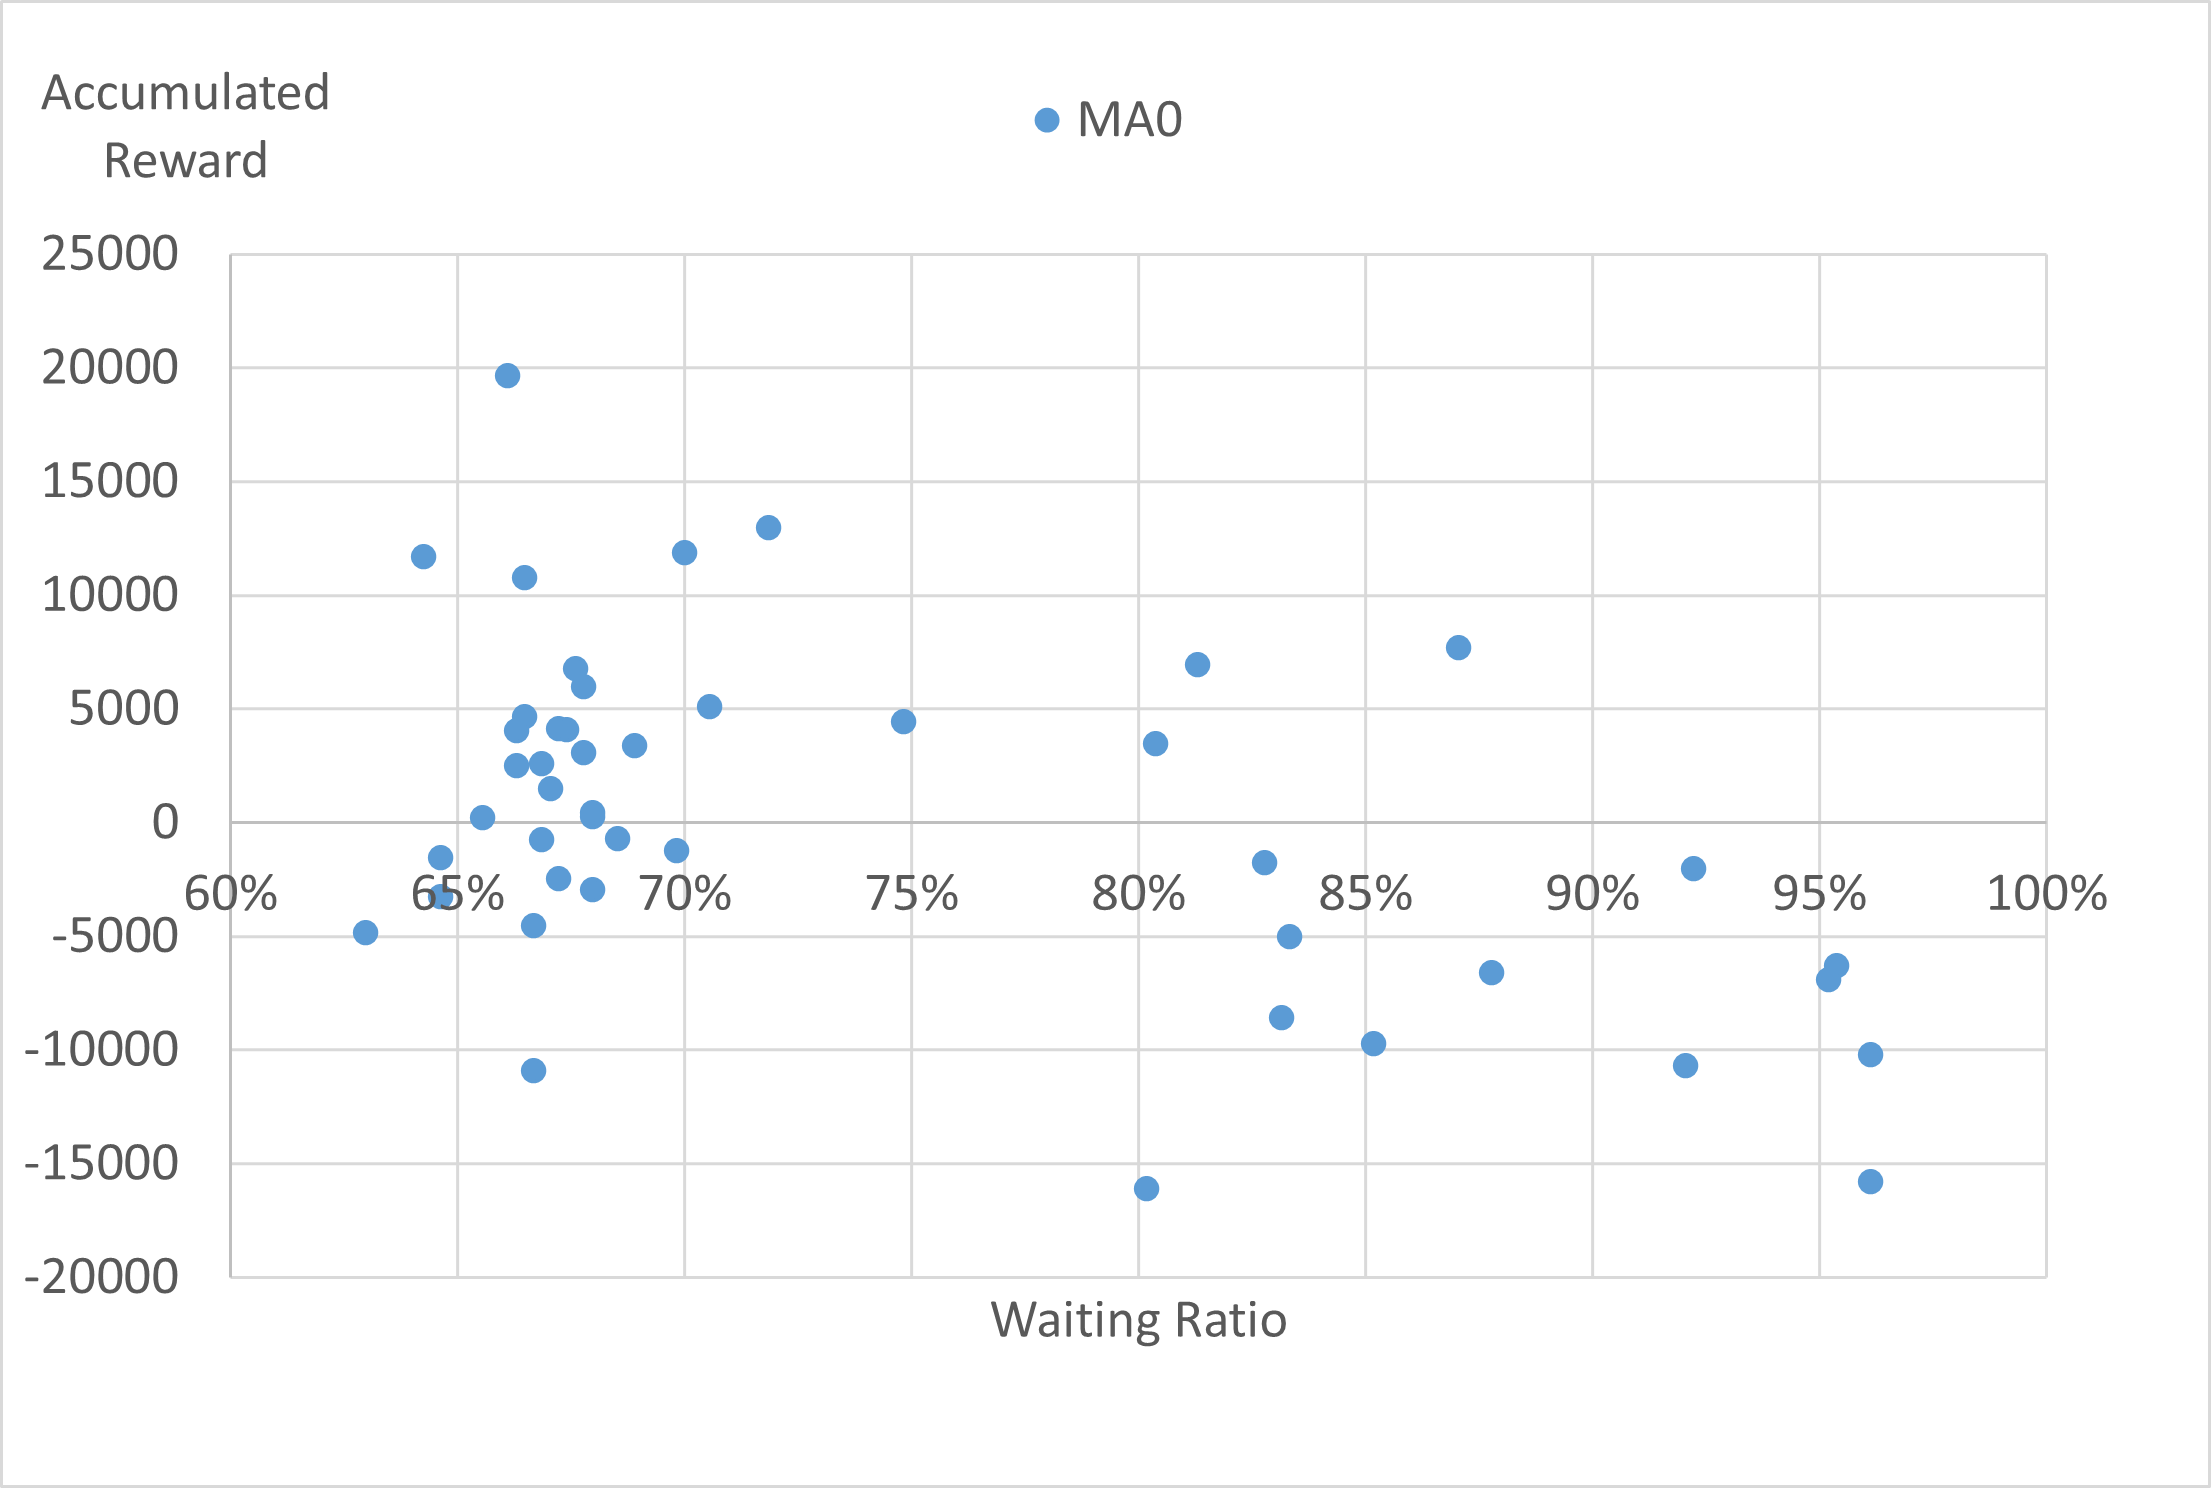
\includegraphics[scale=0.5]{./Figure/ma0waitingReward.png}
  \caption{Scatter plot between waiting ratio and accumulated reward in training of MA0}
  \label{fig:ma0waitingReward}
\end{figure}

\begin{figure}[htbp]
  \centering
  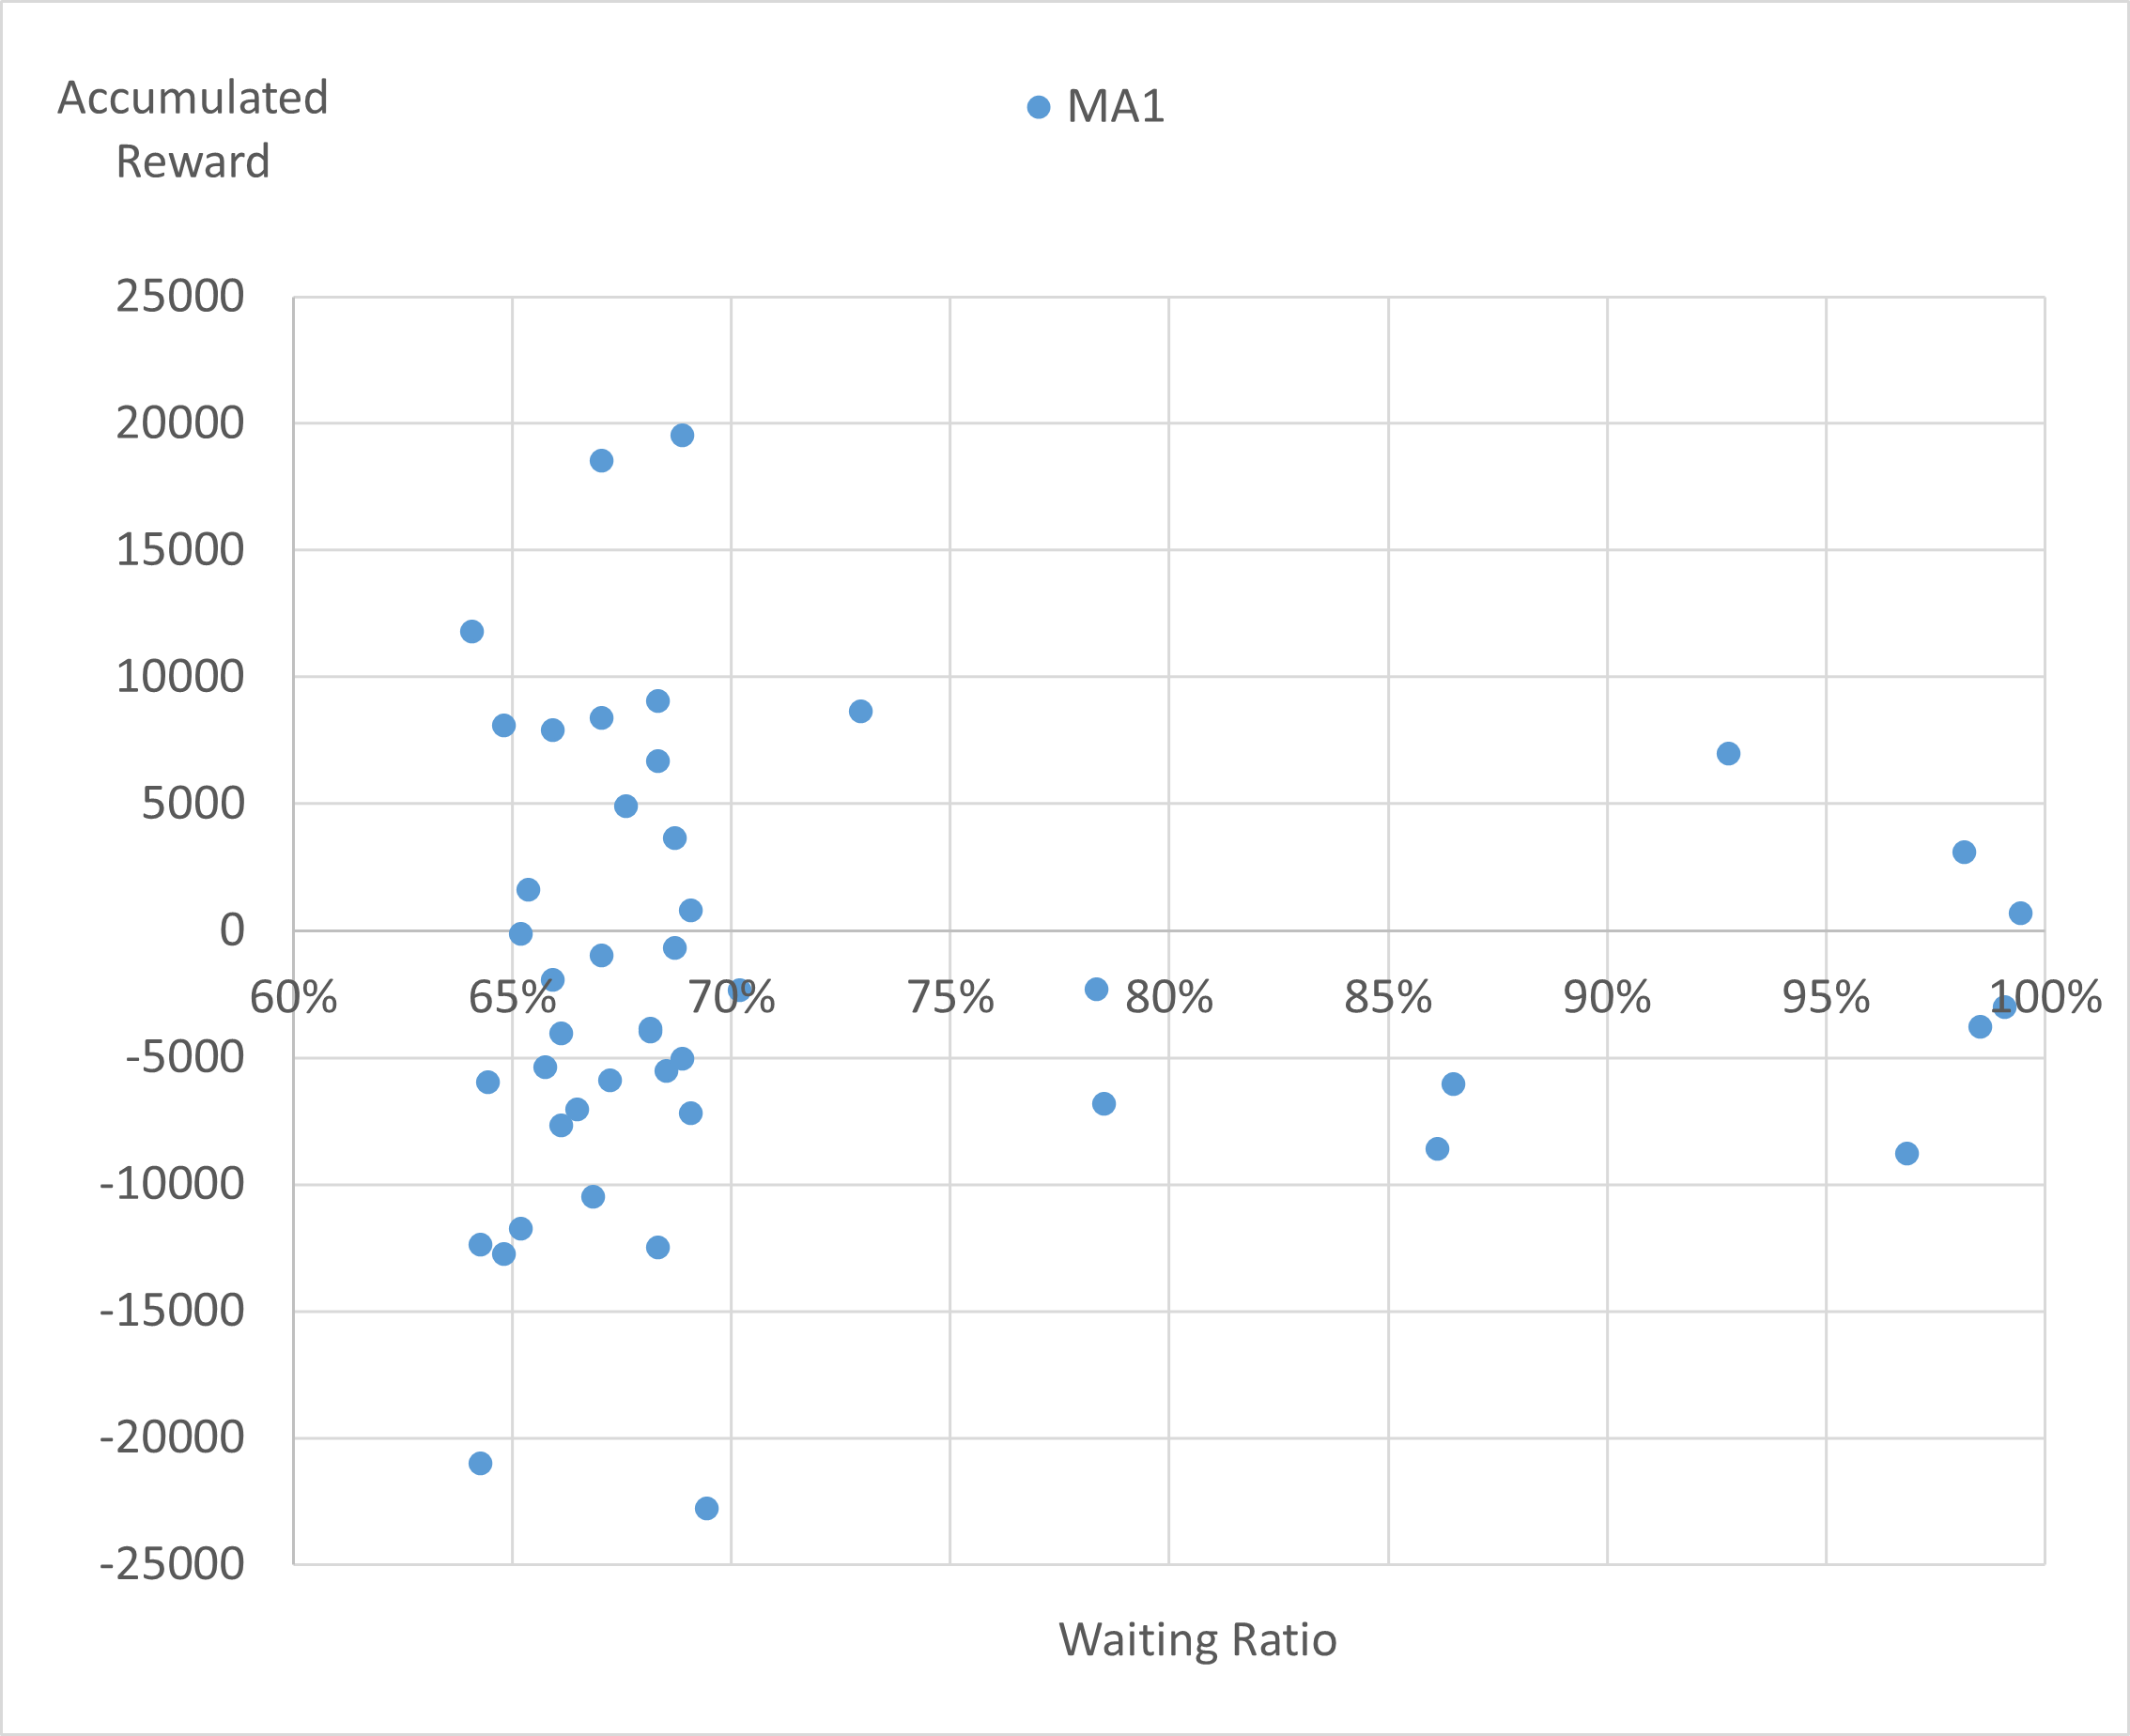
\includegraphics[scale=0.5]{./Figure/ma1waitingReward.png}
  \caption{Scatter plot between waiting ratio and accumulated reward in training of MA1}
  \label{fig:ma1waitingReward}
\end{figure}

\begin{figure}[htbp]
  \centering
  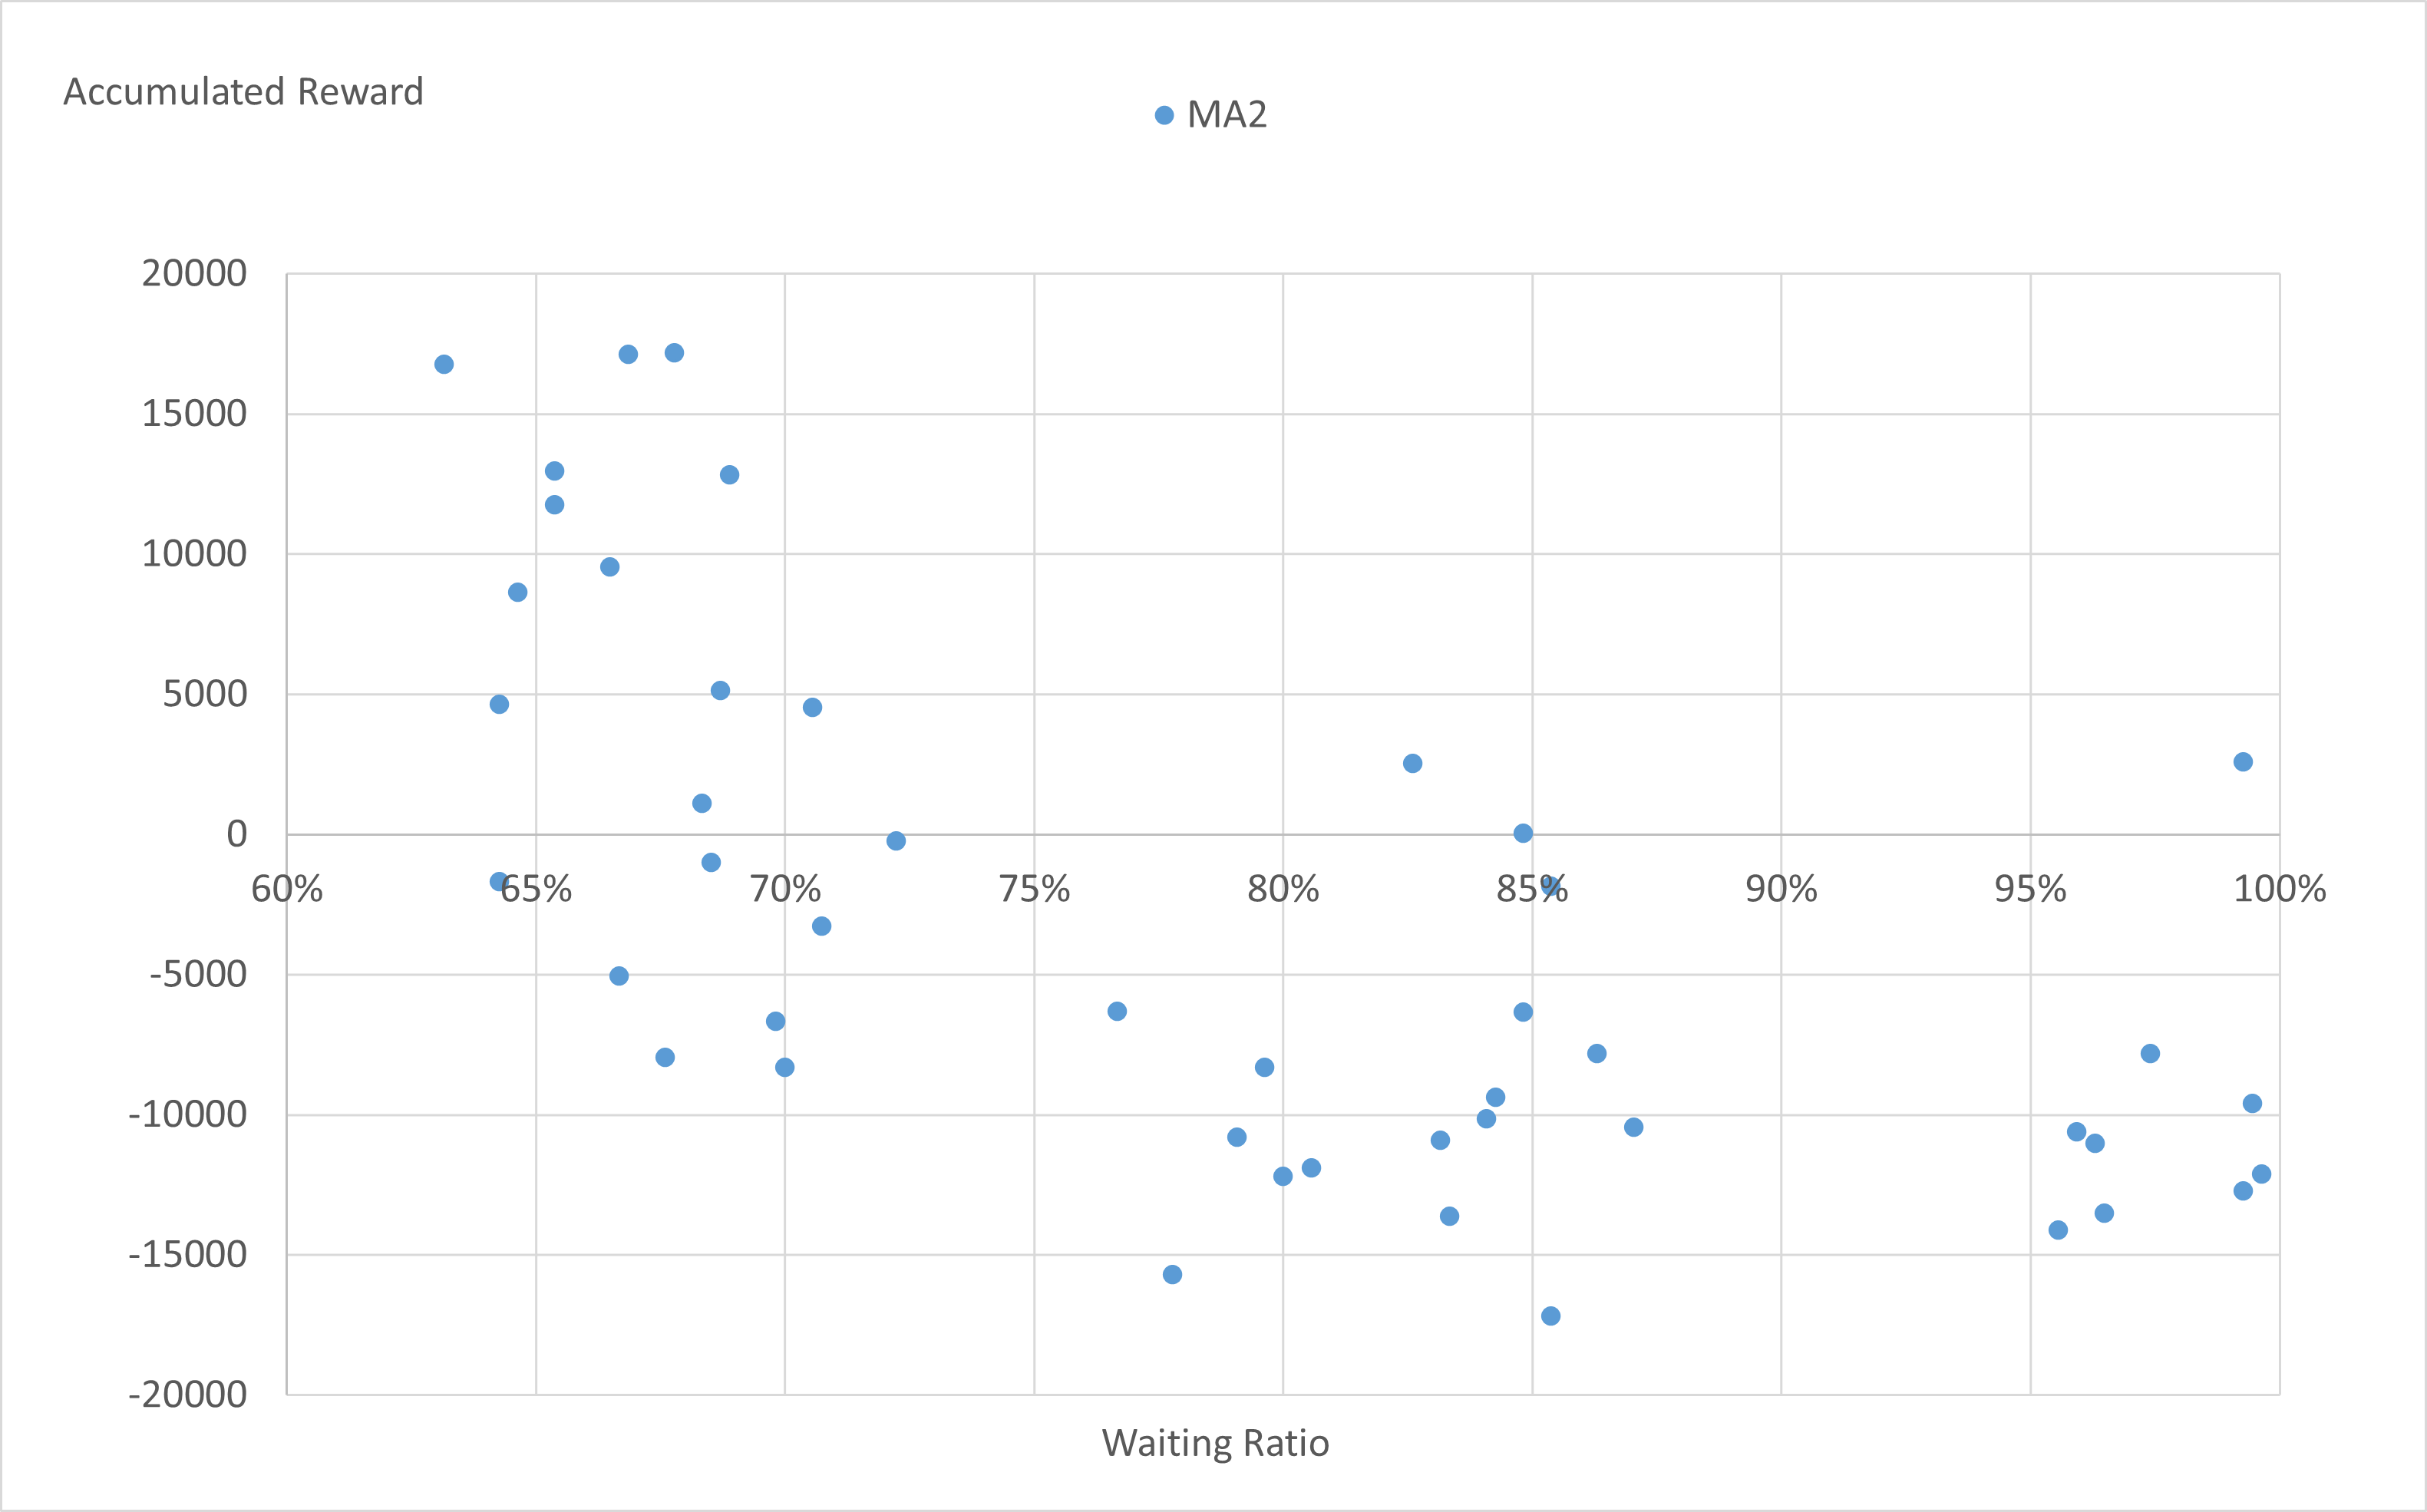
\includegraphics[scale=0.5]{./Figure/ma2waitingReward.png}
  \caption{Scatter plot between waiting ratio and accumulated reward in training of MA2}
  \label{fig:ma2waitingReward}
\end{figure}

\begin{figure}[htbp]
  \centering
  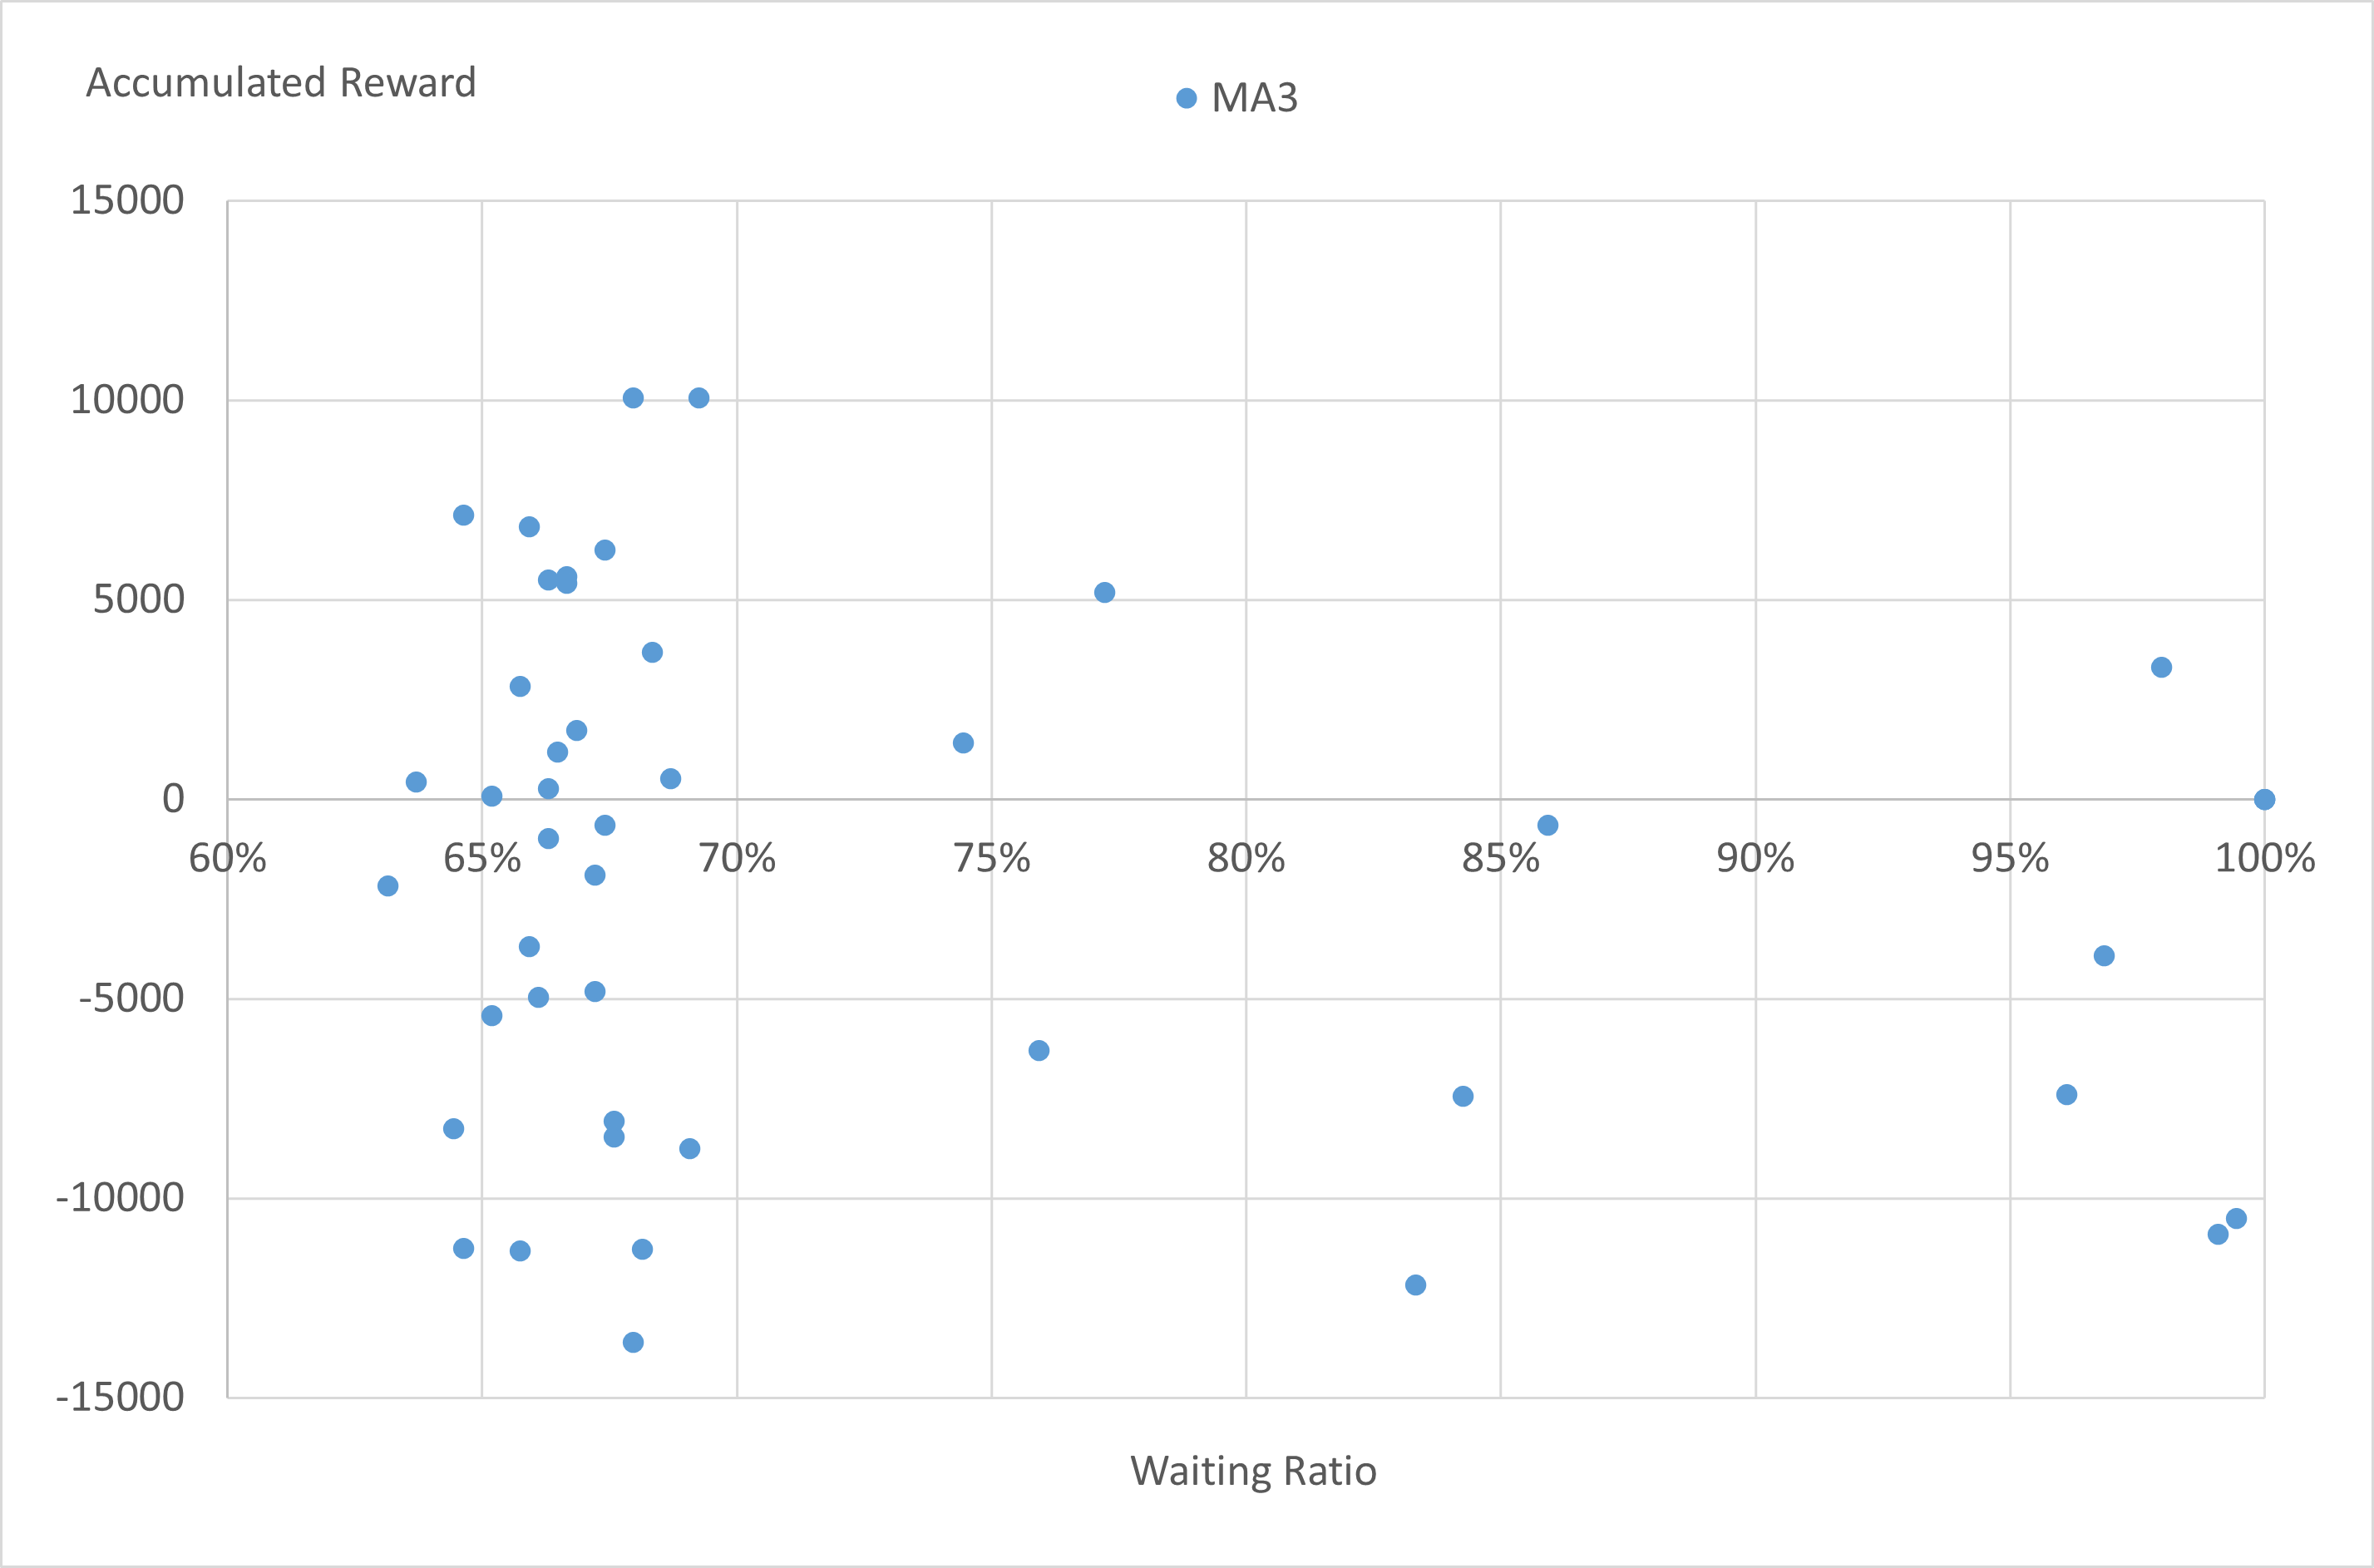
\includegraphics[scale=0.5]{./Figure/ma3waitingReward.png}
  \caption{Scatter plot between waiting ratio and accumulated reward in training of MA3}
  \label{fig:ma3waitingReward}
\end{figure}

\begin{figure}[htbp]
  \centering
  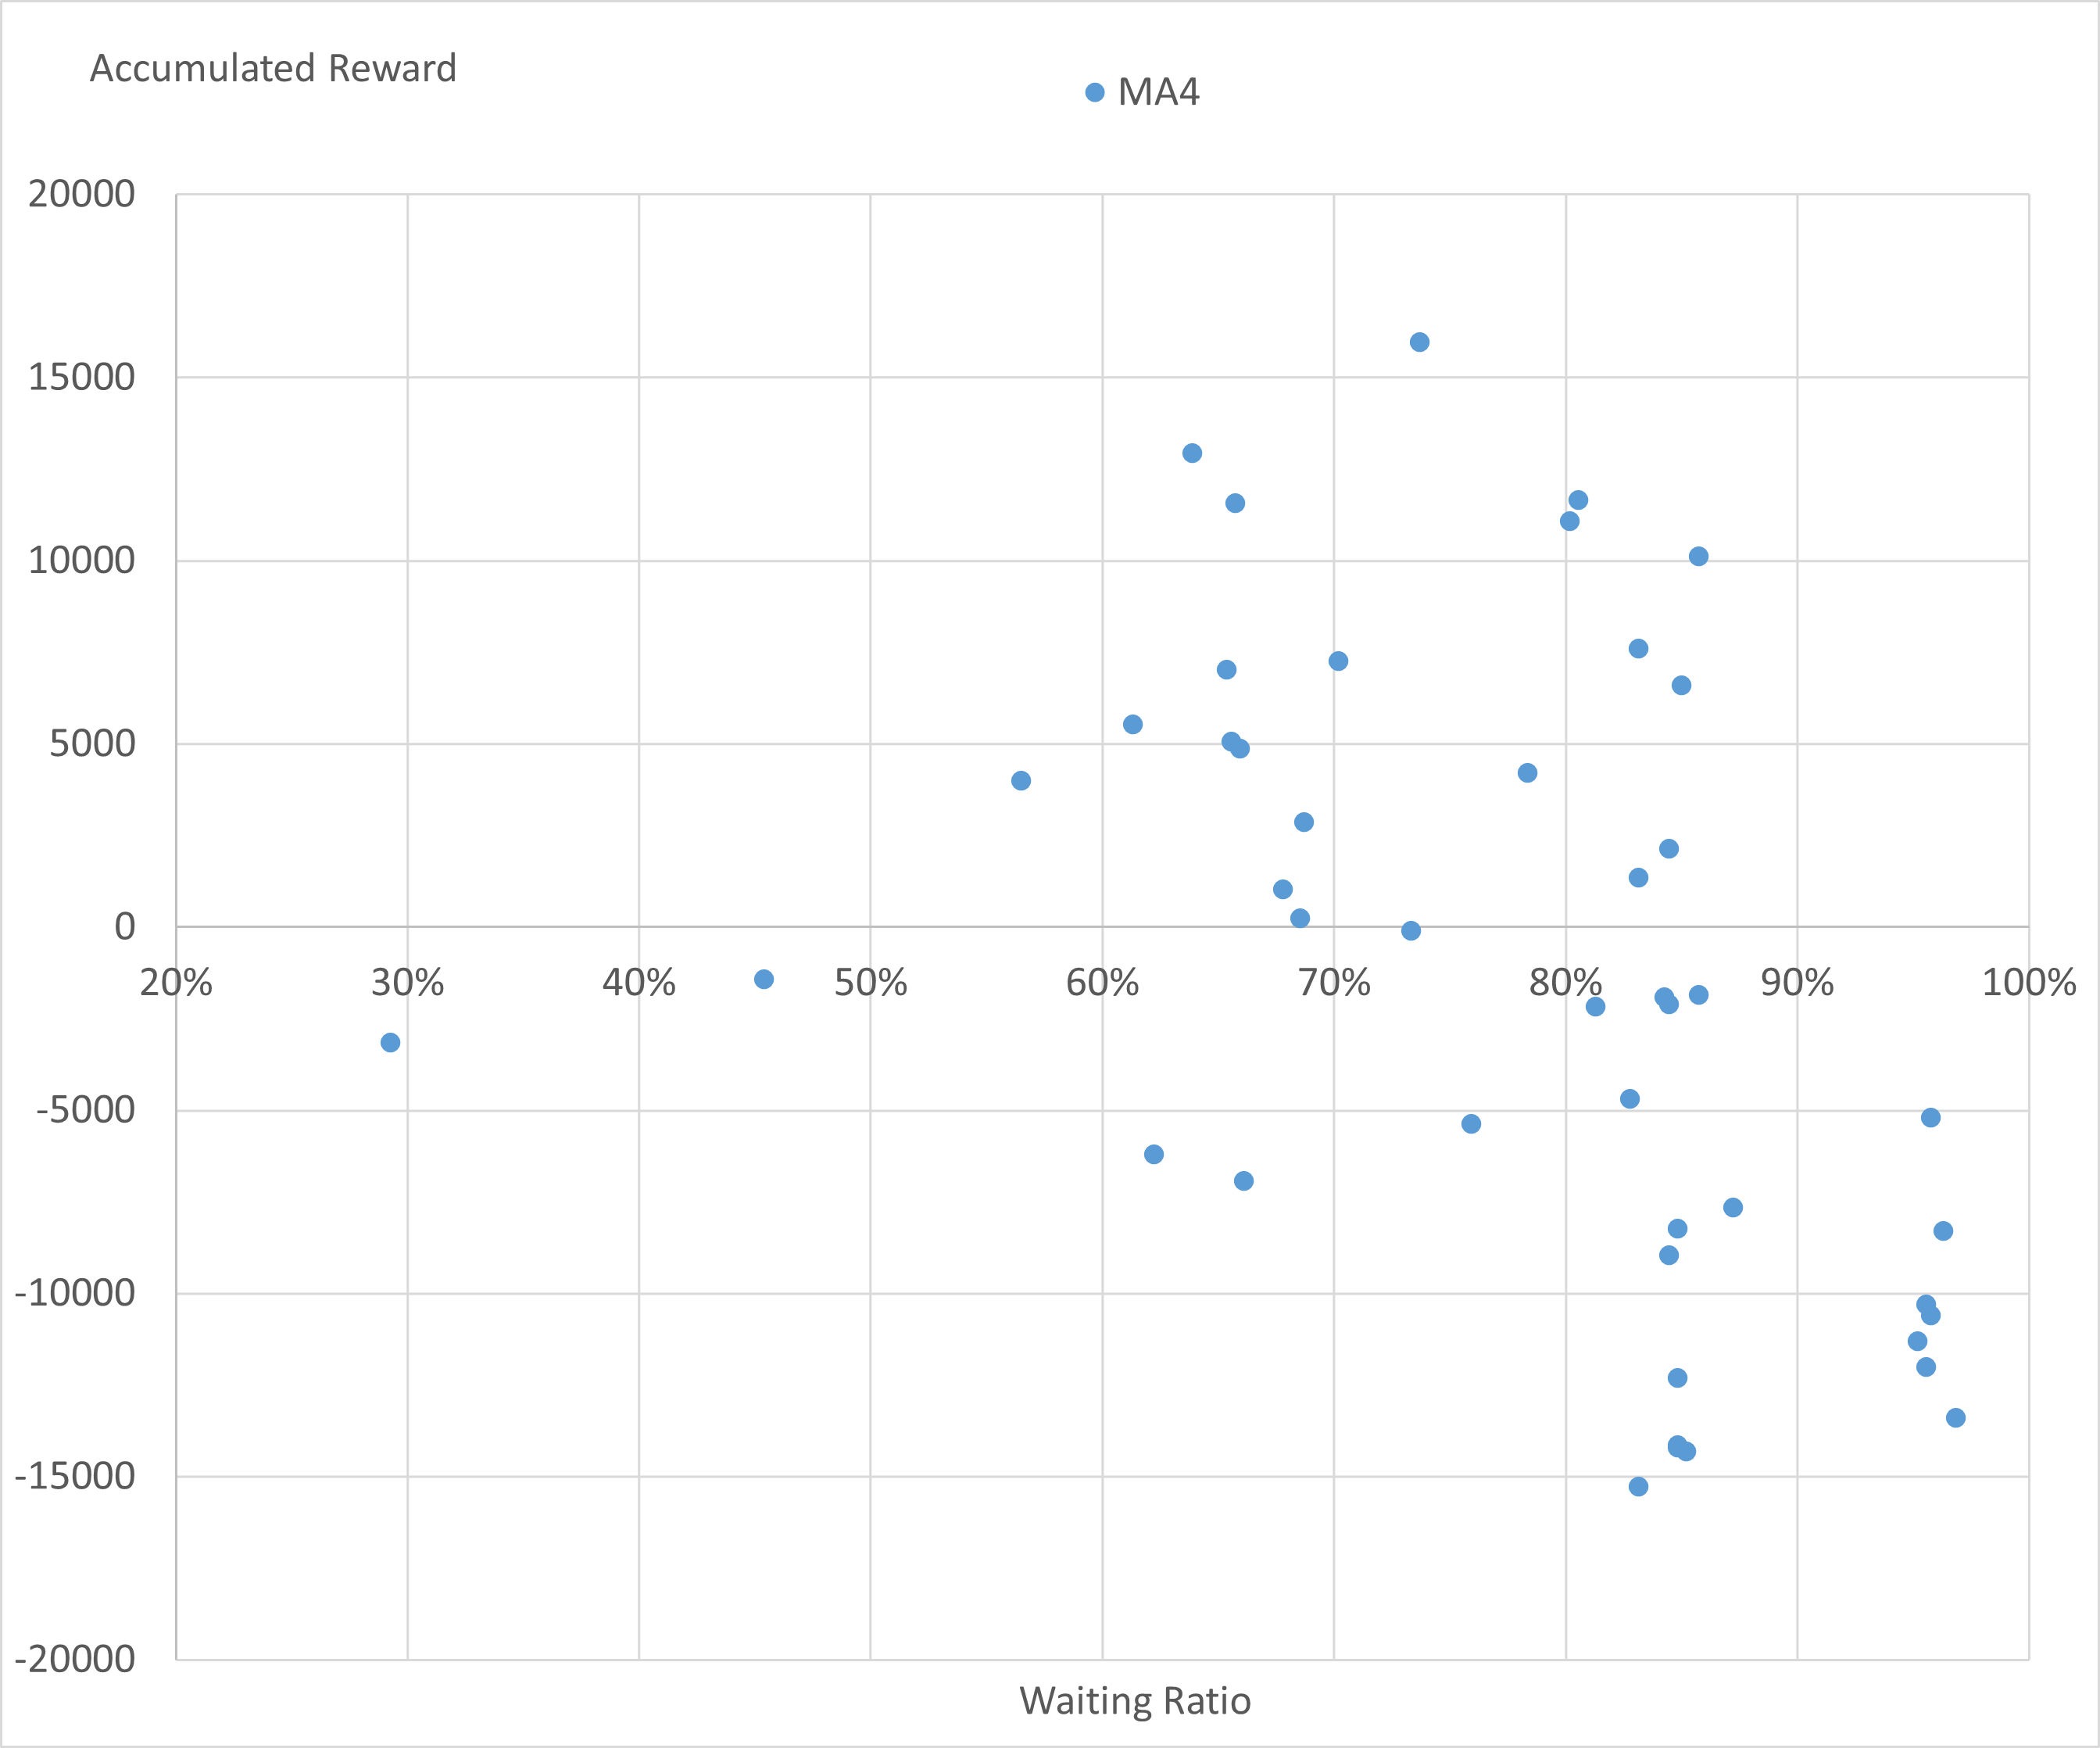
\includegraphics[scale=0.5]{./Figure/ma4waitingReward.png}
  \caption{Scatter plot between waiting ratio and accumulated reward in training of MA4}
  \label{fig:ma4waitingReward}
\end{figure}

\begin{figure}[htbp]
  \centering
  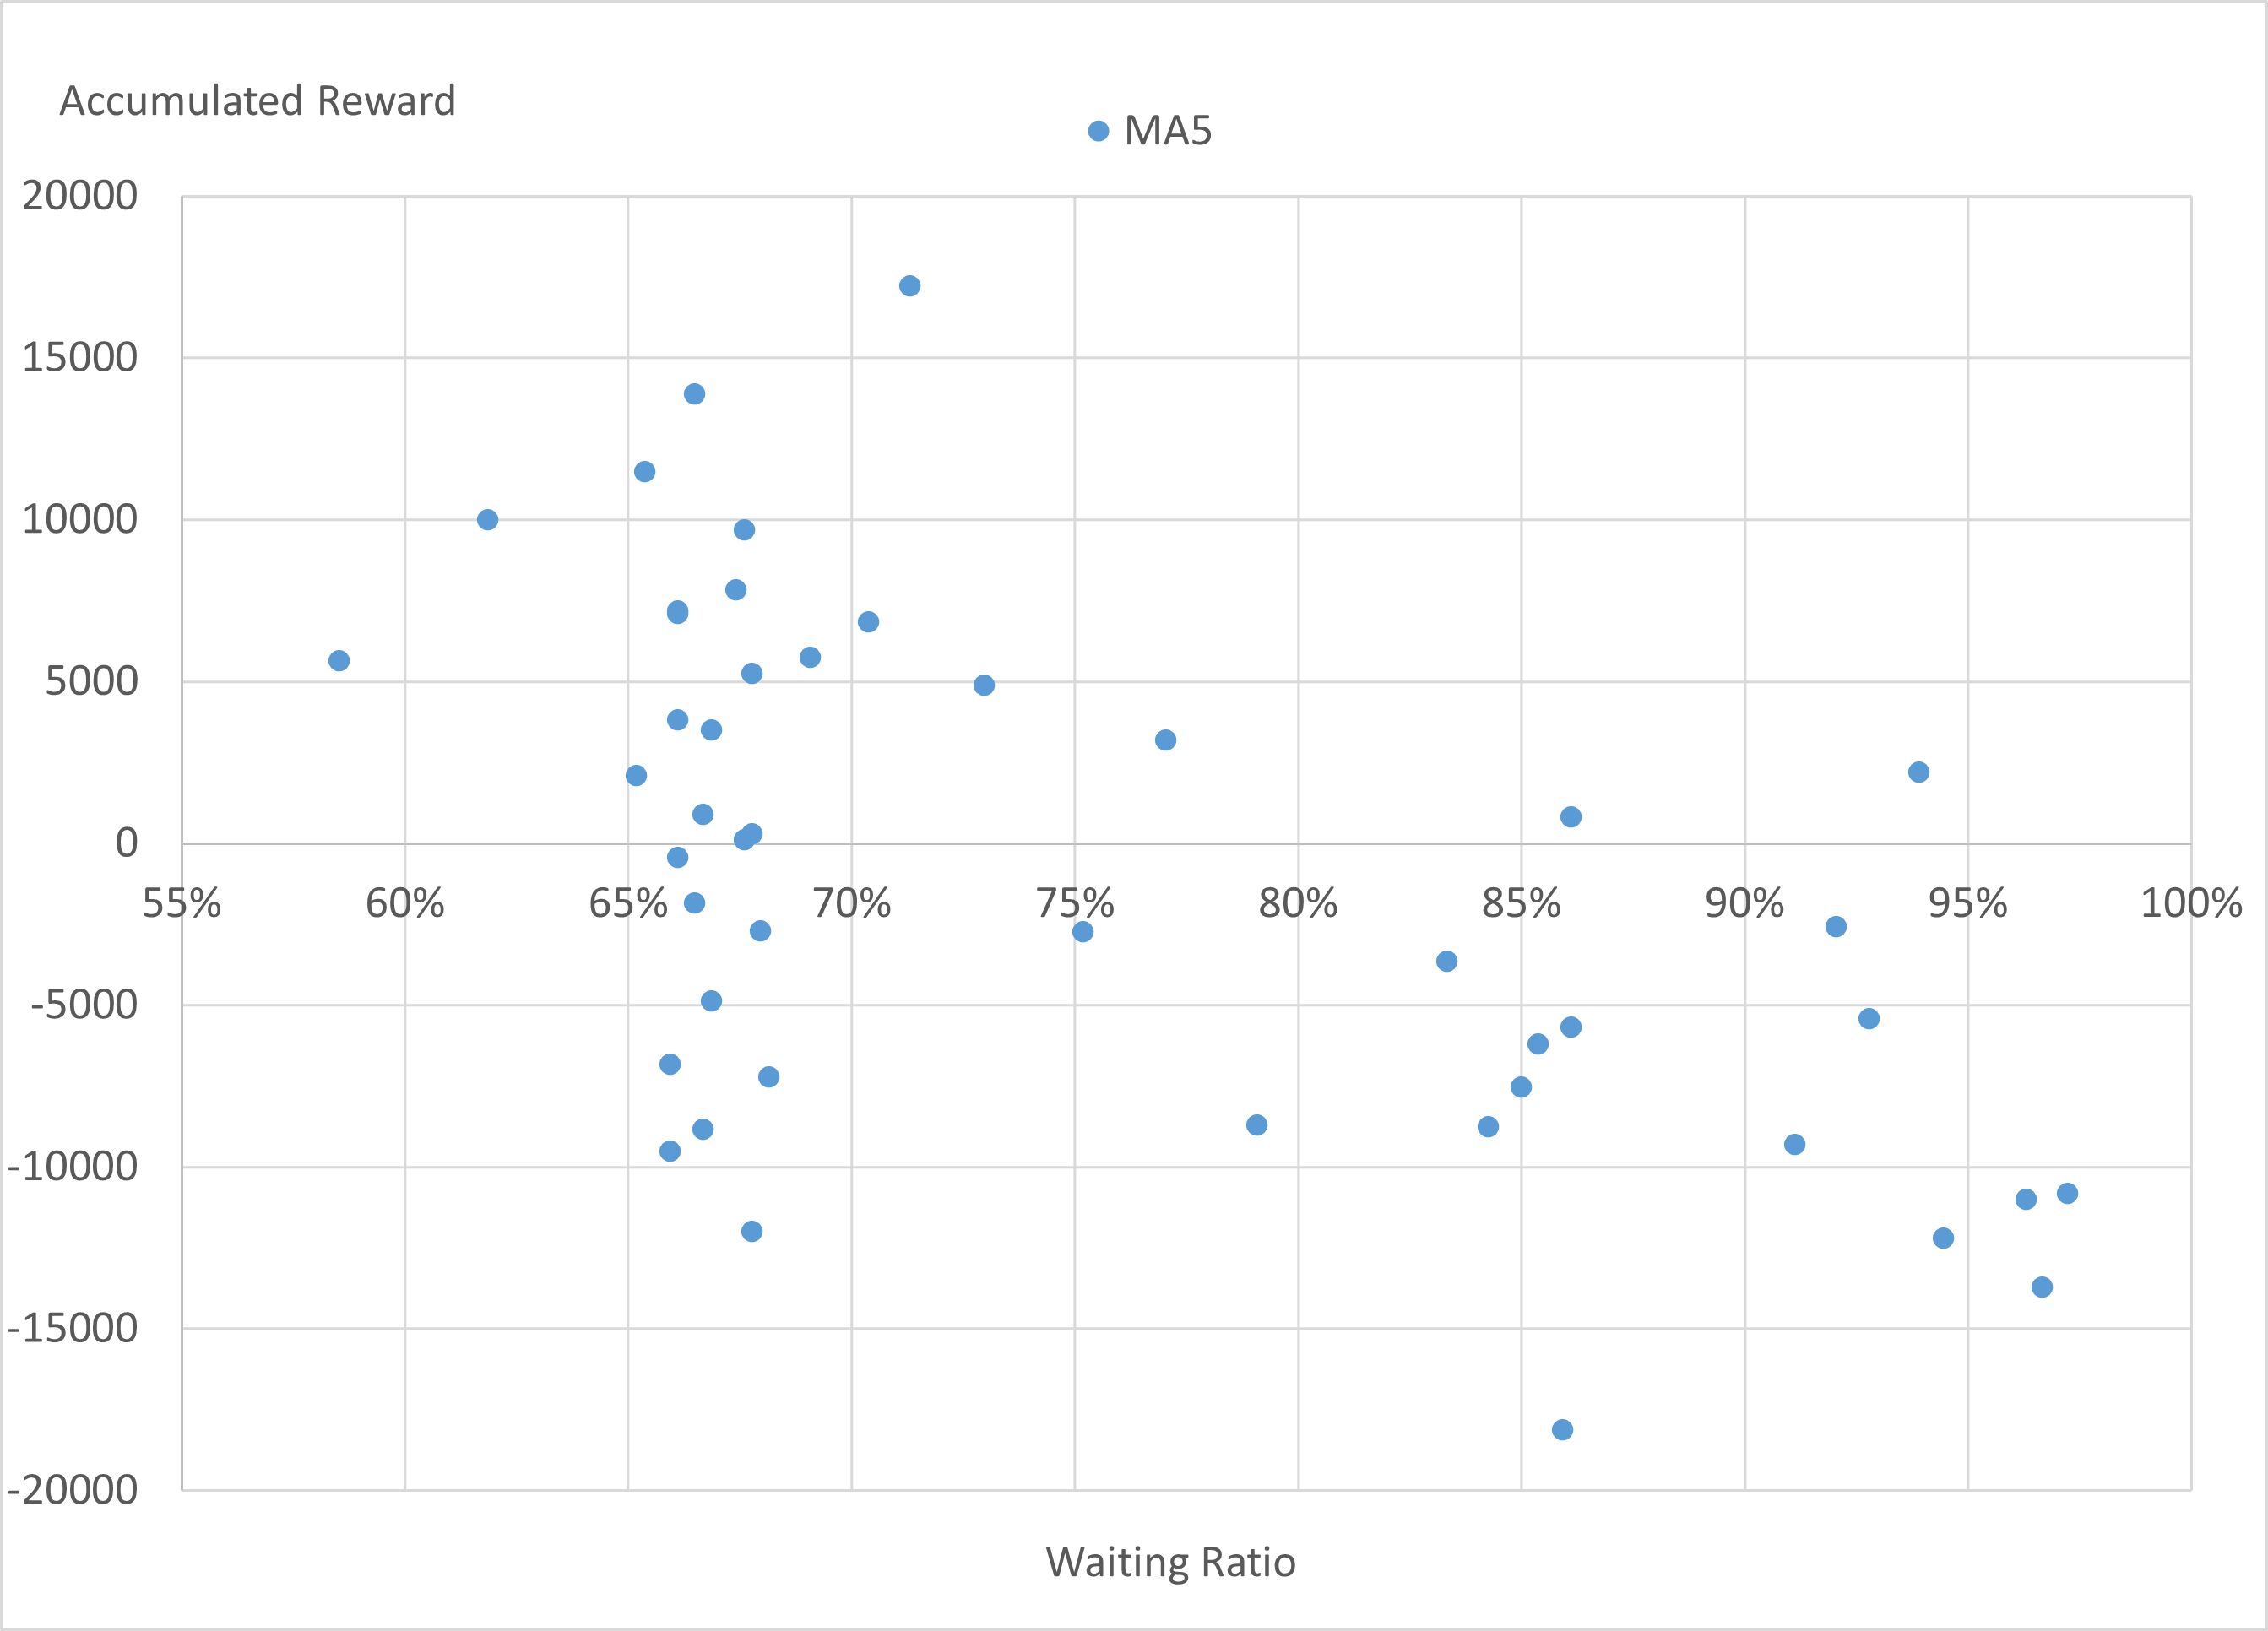
\includegraphics[scale=0.5]{./Figure/ma5waitingReward.png}
  \caption{Scatter plot between waiting ratio and accumulated reward in training of MA5}
  \label{fig:ma5waitingReward}
\end{figure}

Figure \ref{fig:waitingTest} and \ref{fig:waitingTestAvg} are consistent with the expectation of Section \ref{sec:evaluation}: the further the period of testing dataset is from the training period, the more the waiting ratio increases. The waiting can prevent losses when the agent cannot expect the future exchange rate.

In conclusion, RL itself is considered to be useful for avoiding losses in Forex trading.

\begin{figure}[htbp]
  \centering
  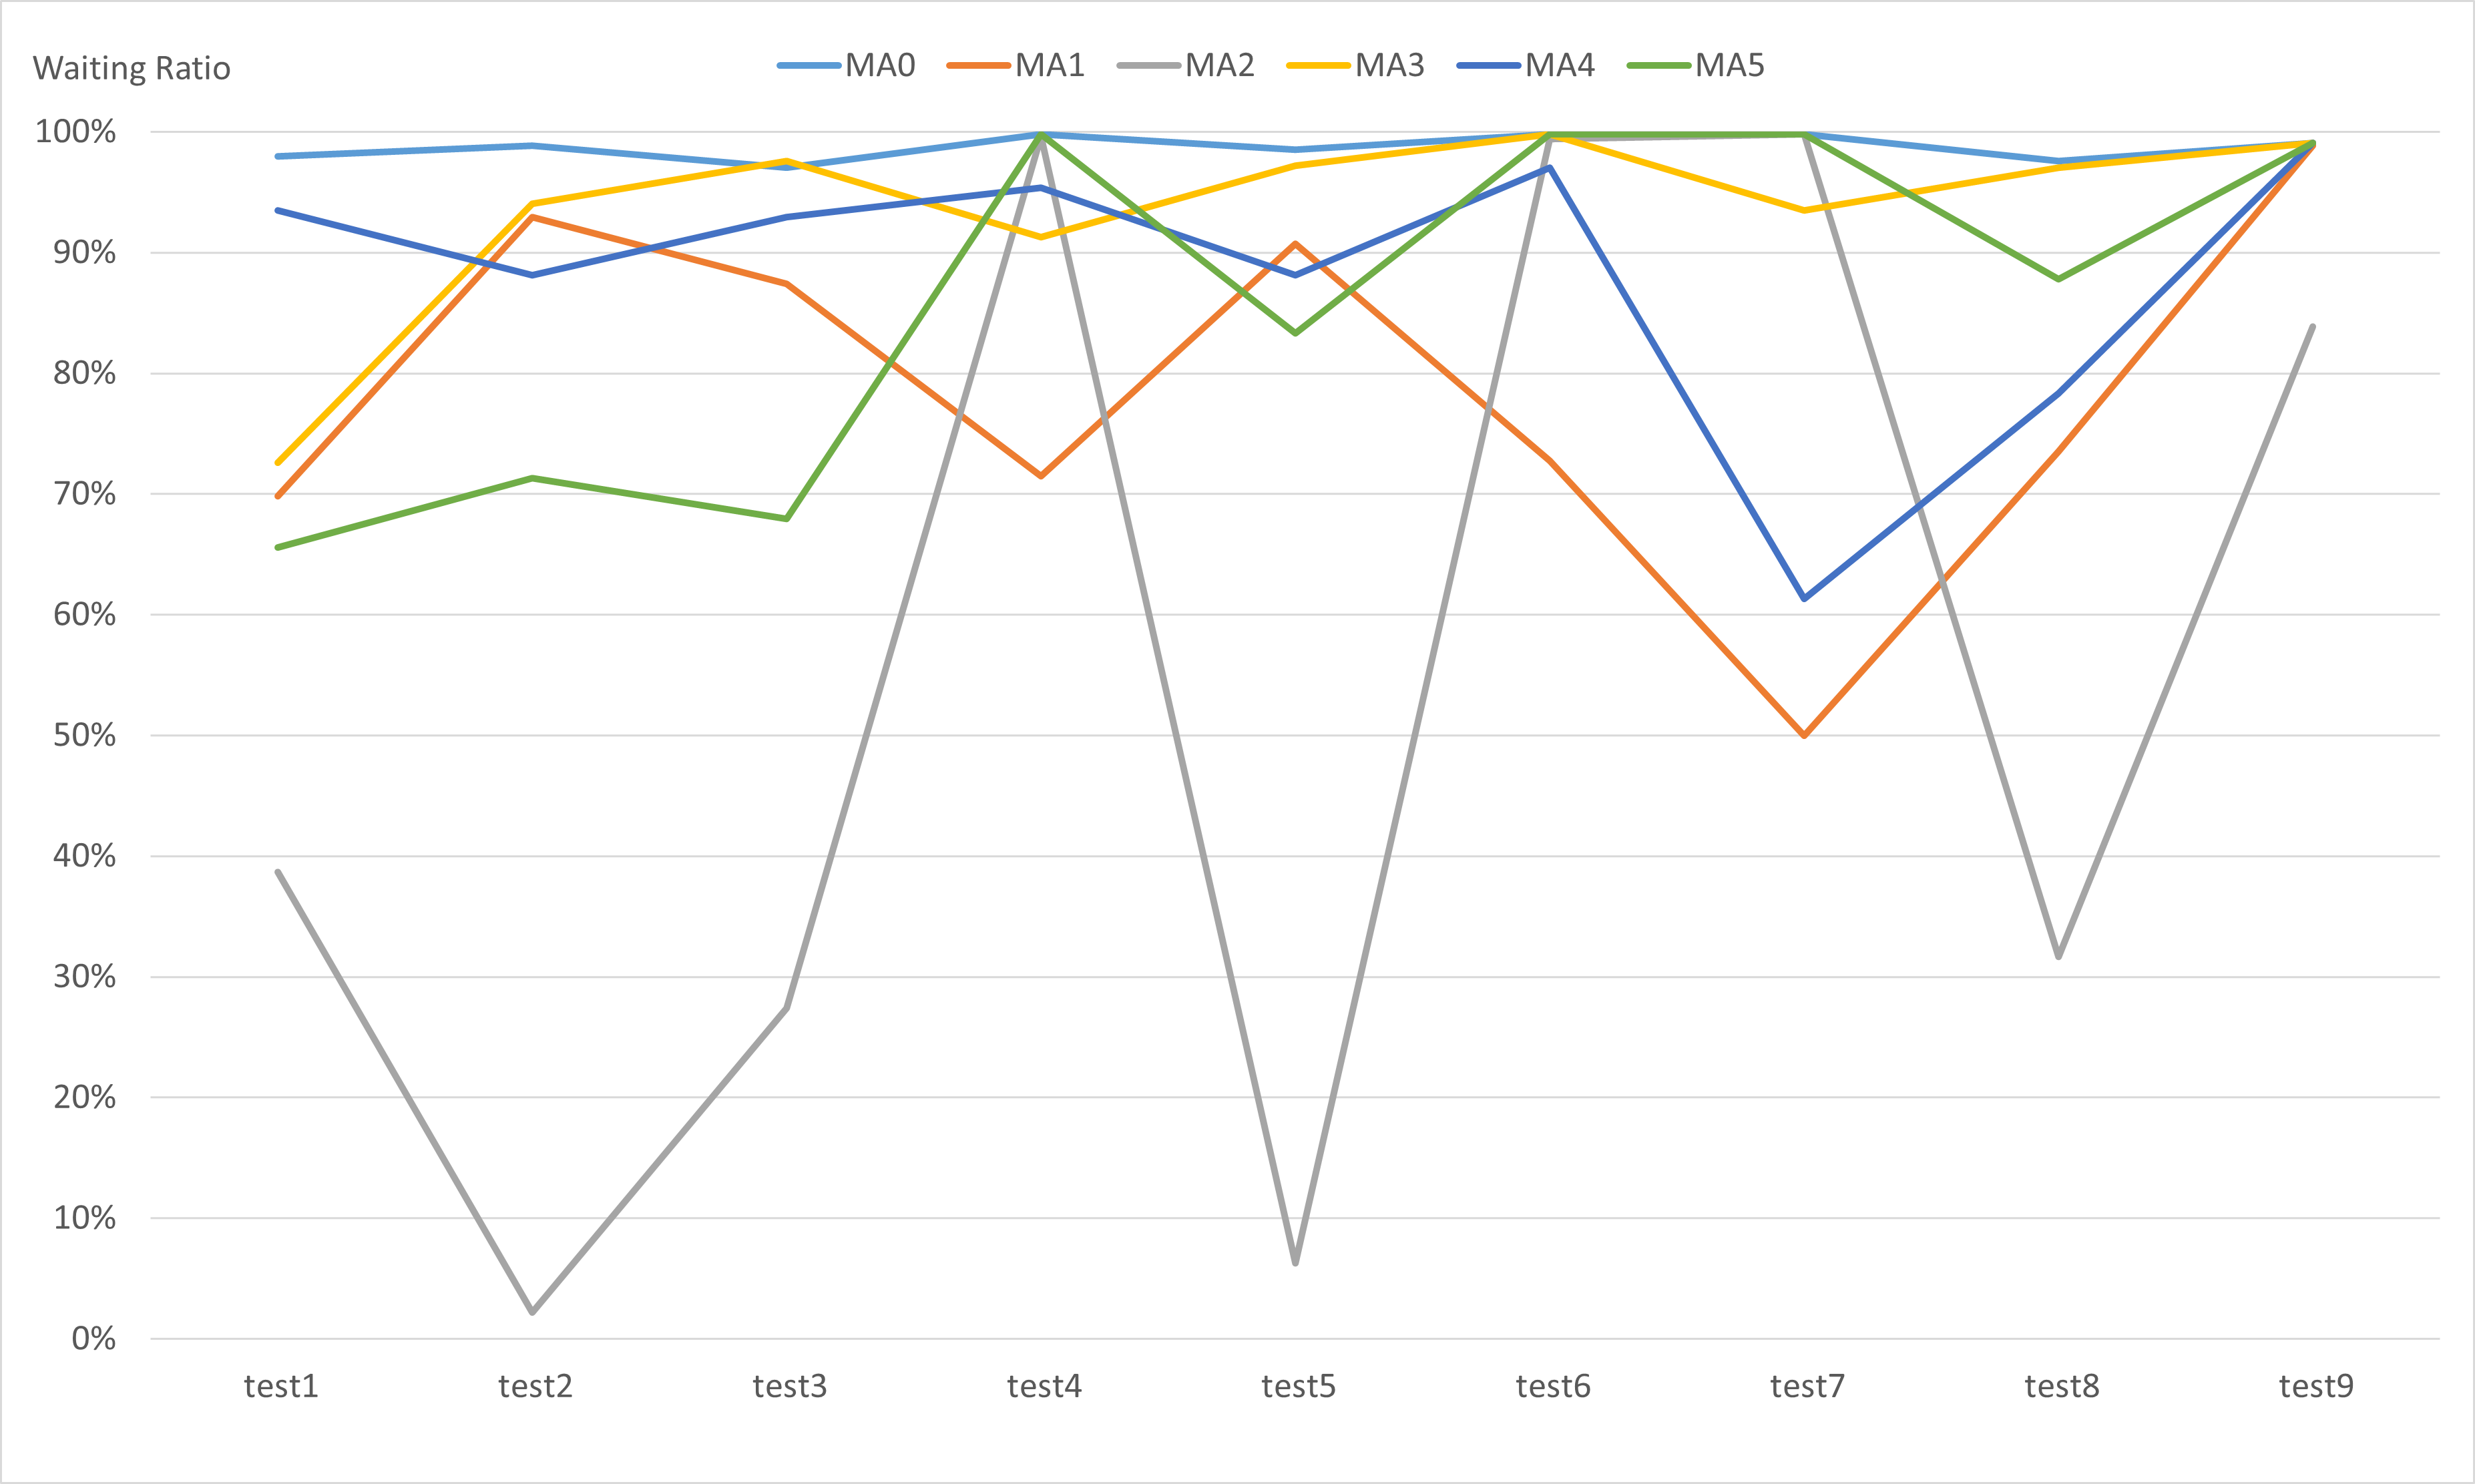
\includegraphics[scale=0.5]{./Figure/waitingTest.png}
  \caption{Waiting ratio in testing for the number of MA}
  \label{fig:waitingTest}
\end{figure}

\begin{figure}[htbp]
  \centering
  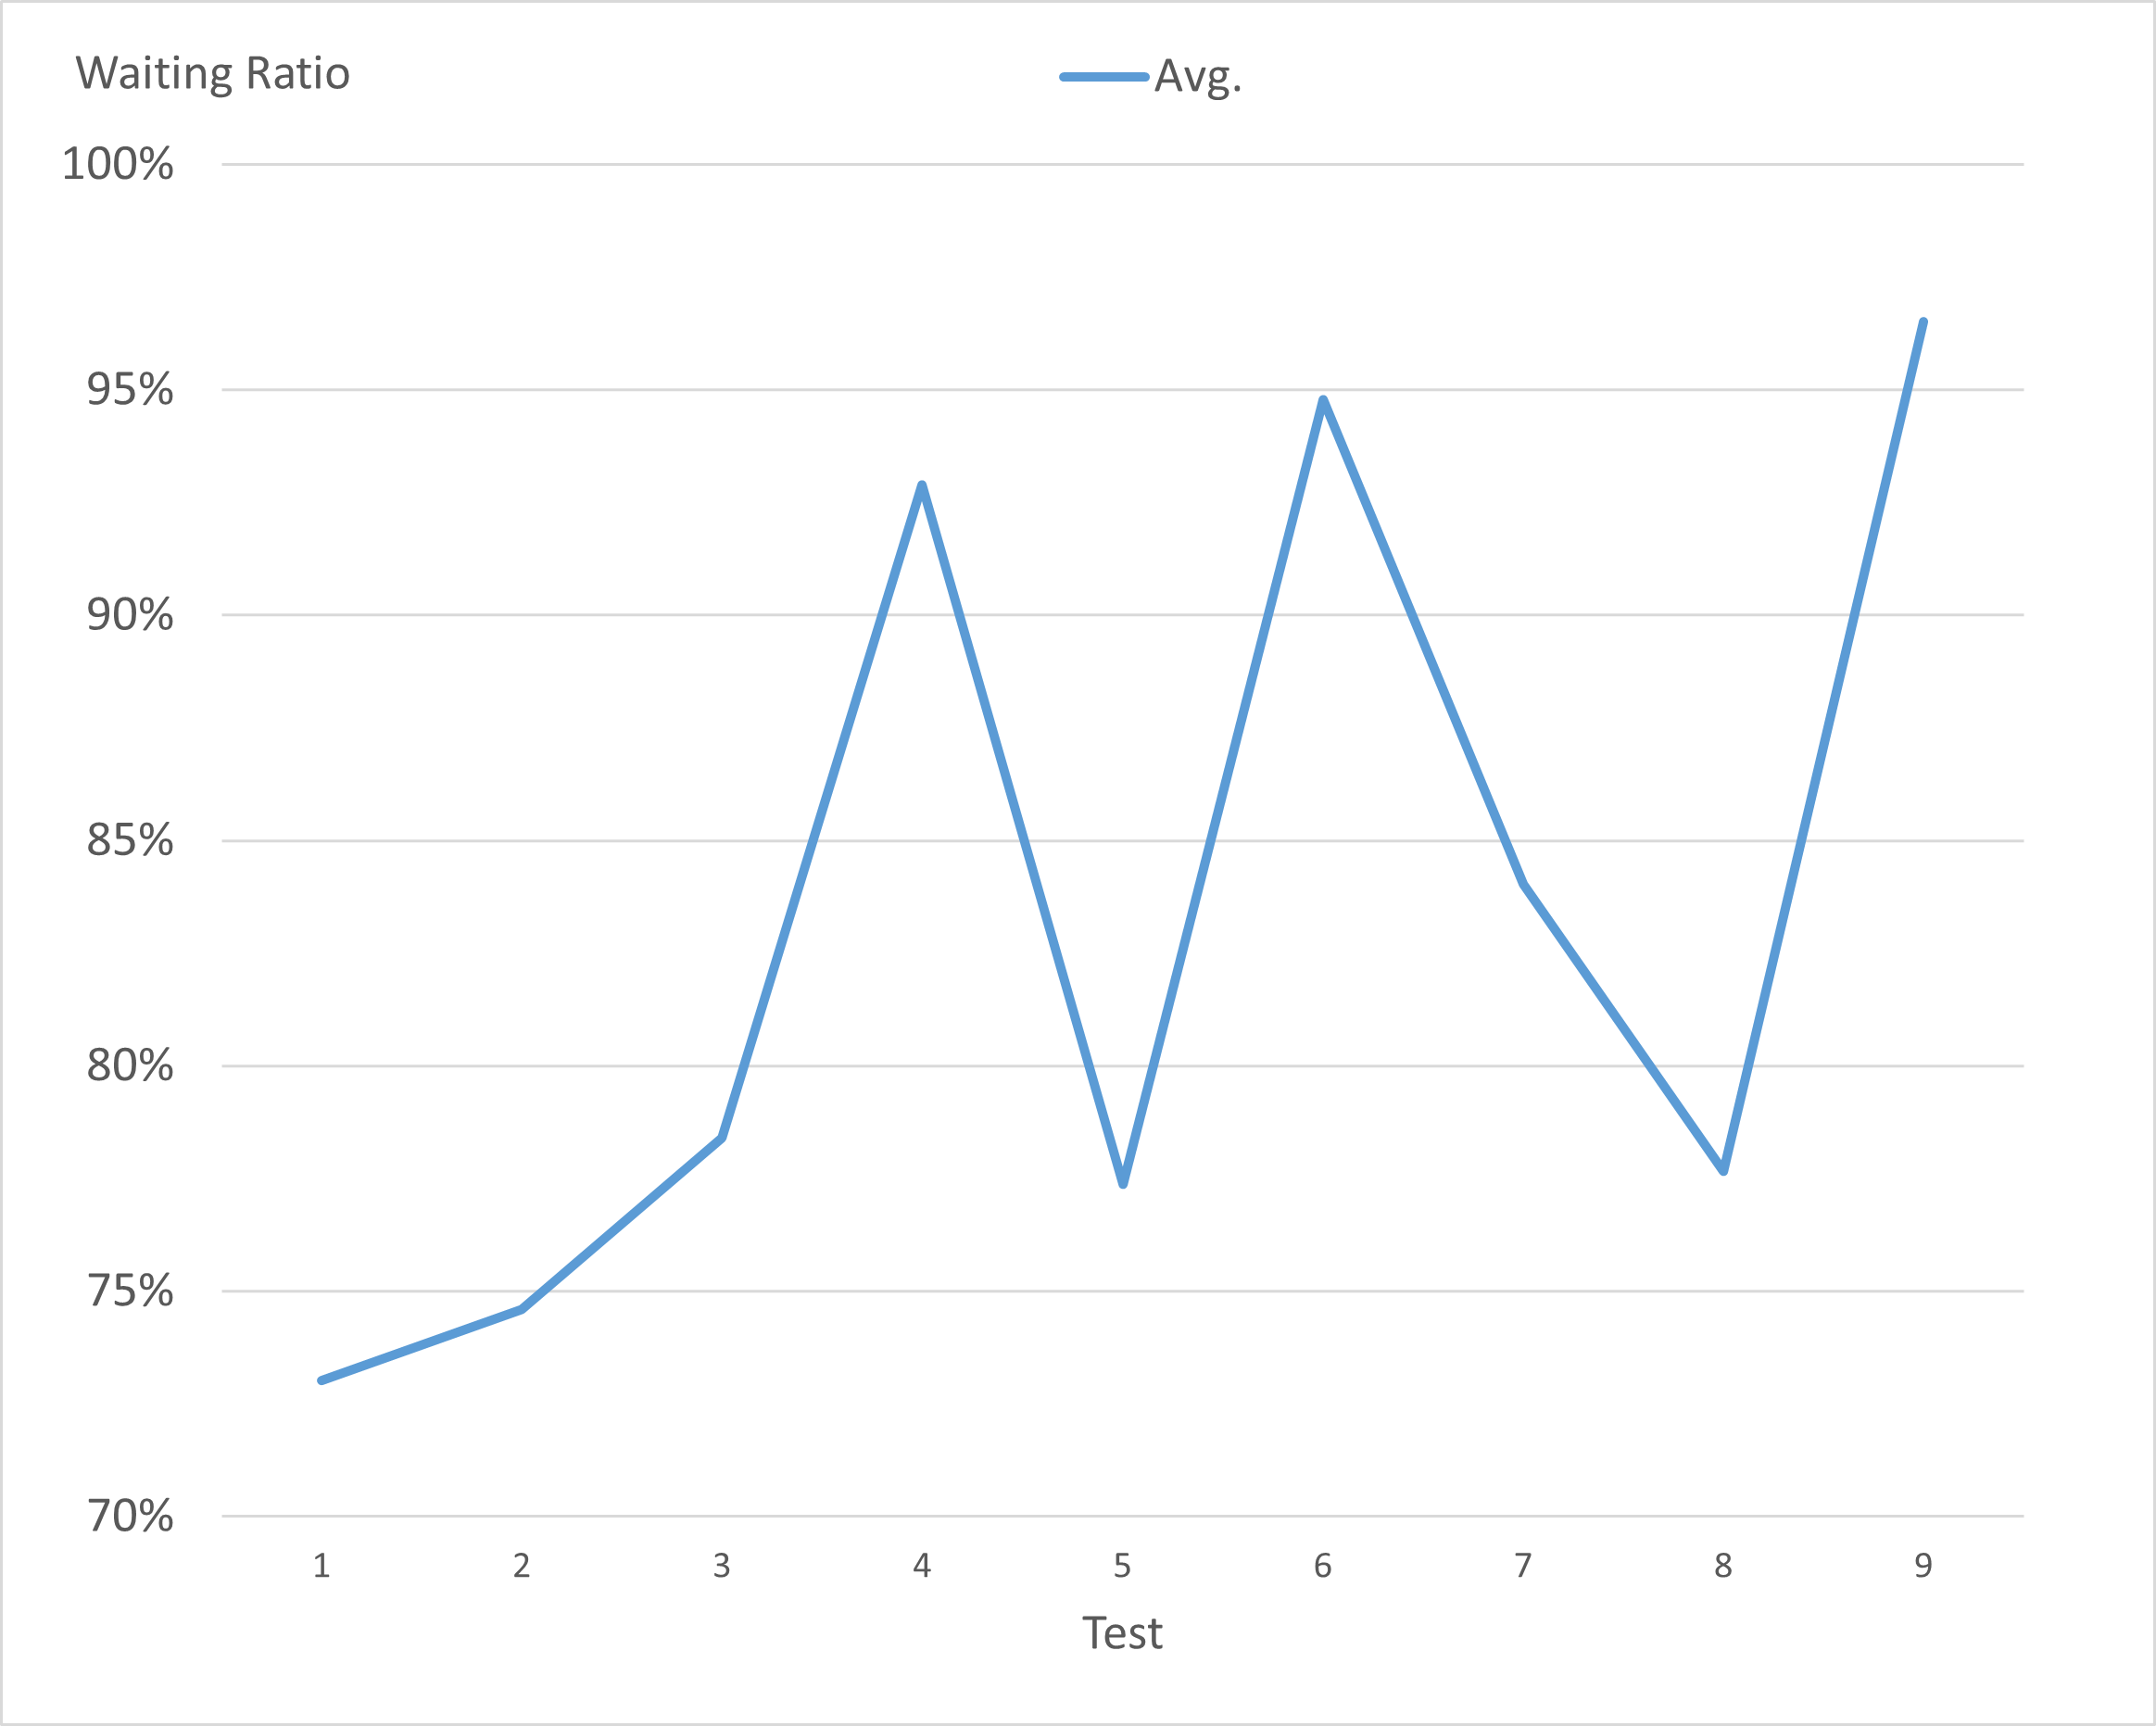
\includegraphics[scale=0.6]{./Figure/waitingTestAvg.png}
  \caption{Average of waiting ratio in testing}
  \label{fig:waitingTestAvg}
\end{figure}

\chapter{Conclusion}
\label{sec:conclusion}
According to the result of the accumulation reward, the experiments could not prove the importance of multiple MAs. We concluded that MA may be invalid metrics for DQL of Forex trading. However, it is difficult to assert that MA is invalid metrics as state element because professional financial analysts still utilize it. Other causes of this research may prevent the performance. For example, hyperparameter such as step may be inappropriate or the way of utilizing MA may be too simple to perform for Forex trading. 

On the other hand, the result of the waiting ratio suggested that RL itself can be useful to avoid losses.

The biggest problem was that the agent failed to learn to get profit in both training and testing. Unfortunately, my research method was not useful for an algorithmic trading system.

Further investigations are needed to make this DQN method practical. Firstly, we have to decide whether MA is invalid metrics for Forex trading with the experiments to vary hyperparameters, the way of utilizing MA, and the type of DQN. After that, if it turns out that MA is invalid, we have to consider other metrics. For example, oscillator, Fibonacci retracement, relative strength index (RSI), or Bollinger Band can be the candidate of it \cite{analysisMetrics}. In addition, we may need to consider combining DQL with the price prediction model such as using convolutional neural network (CNN) \cite{Suchaimanacharoen2020}.

Secondly, as Section \ref{sec:actMod} suggested, the agent with DQN is supposed to skip learning the position transition since the transition is deterministic. Therefore, we will have to find the way to realize it while DQN focuses on a stochastic environment.

Lastly, we have to verify whether RL actually avoids losses in the trading. Section \ref{sec:waitingRatioResult} suggested the RL usefulness, but it was not enough to prove it. To validate the evidence, we must also identify which statistics need to be analyzed.


% % %
% End of Body
% % %

% % Bibliography style
\singlespacing
\bibliographystyle{IEEEtran}
\bibliography{ref}
% % If you add references to a table of contents, uncomment the following line
\addcontentsline{toc}{chapter}{References}

% % You can make appendixes, if any.
% \appendix
% \include{./Chapter/hogehoge.tex}

\end{document}
